\pdfoutput=1

\documentclass{l4proj}
\usepackage[english]{babel}
\usepackage[utf8]{inputenc}
\usepackage{amsmath}
\usepackage{listings}
\usepackage{graphicx}
\usepackage{url}
\usepackage{xcolor}
\usepackage{hyperref}
\usepackage{amsmath}
\usepackage{cleveref}
\usepackage{dirtree}
\usepackage{subfigure}

\hypersetup{
  colorlinks   = true, %Colours links instead of ugly boxes
  urlcolor     = blue, %Colour for external hyperlinks
  linkcolor    = blue, %Colour of internal links
  citecolor   = black %Colour of citations
}

\colorlet{punct}{red!60!black}
\definecolor{lightgray}{rgb}{0.95, 0.95, 0.95}
\definecolor{darkgray}{rgb}{0.4, 0.4, 0.4}
%\definecolor{purple}{rgb}{0.65, 0.12, 0.82}
\definecolor{editorGray}{rgb}{0.95, 0.95, 0.95}
\definecolor{editorOcher}{rgb}{1, 0.5, 0} % #FF7F00 -> rgb(239, 169, 0)
\definecolor{editorGreen}{rgb}{0, 0.5, 0} % #007C00 -> rgb(0, 124, 0)
\definecolor{orange}{rgb}{1,0.45,0.13}    
\definecolor{olive}{rgb}{0.17,0.59,0.20}
\definecolor{brown}{rgb}{0.69,0.31,0.31}
\definecolor{purple}{rgb}{0.38,0.18,0.81}
\definecolor{lightblue}{rgb}{0.1,0.57,0.7}
\definecolor{lightred}{rgb}{1,0.4,0.5}
\definecolor{background}{HTML}{EEEEEE}
\definecolor{delim}{RGB}{20,105,176}
\colorlet{numb}{magenta!60!black}
%V8 C++
\lstdefinelanguage{cpp}{
  morekeywords={typeof, new, true, false, catch, function, return, null, catch, switch, var, if, in, while, do, else, case, break,Isolate,CreateParams,New},
  morecomment=[s]{/*}{*/},
  morecomment=[l]//,
  morestring=[b]",
  morestring=[b]'
}
% CSS
\lstdefinelanguage{CSS}{
  keywords={color,background-image:,margin,padding,font,weight,display,position,top,left,right,bottom,list,style,border,size,white,space,min,width, transition:, transform:, transition-property, transition-duration, transition-timing-function}, 
  sensitive=true,
  morecomment=[l]{//},
  morecomment=[s]{/*}{*/},
  morestring=[b]',
  morestring=[b]",
  alsoletter={:},
  alsodigit={-}
}

% JavaScript
\lstdefinelanguage{JavaScript}{
  morekeywords={typeof, new, true, false, catch, function, return, null, catch, switch, var, if, in, while, do, else, case, break},
  morecomment=[s]{/*}{*/},
  morecomment=[l]//,
  morestring=[b]",
  morestring=[b]'
}

\lstdefinelanguage{HTML5}{
  language=html,
  sensitive=true, 
  alsoletter={<>=-},  
  morecomment=[s]{<!-}{-->},
  tag=[s],
  otherkeywords={
  % General
  >,
  % Standard tags
  <!DOCTYPE,
  </html, <html, <head, <title, </title, <style, </style, <link, </head, <meta, />,
  % body
  </body, <body,
  % Divs
  </div, <div, </div>, 
  % Paragraphs
  </p, <p, </p>,
  % scripts
  </script, <script,
  % More tags...
  <canvas, /canvas>, <svg, <rect, <animateTransform, </rect>, </svg>, <video, <source, <iframe, </iframe>, </video>, <image, </image>, <header, </header, <article, </article
  },
  ndkeywords={
  % General
  =,
  % HTML attributes
  charset=, src=, id=, width=, height=, style=, type=, rel=, href=,
  % SVG attributes
  fill=, attributeName=, begin=, dur=, from=, to=, poster=, controls=, x=, y=, repeatCount=, xlink:href=,
  % properties
  margin:, padding:, background-image:, border:, top:, left:, position:, width:, height:, margin-top:, margin-bottom:, font-size:, line-height:,
  % CSS3 properties
  transform:, -moz-transform:, -webkit-transform:,
  animation:, -webkit-animation:,
  transition:,  transition-duration:, transition-property:, transition-timing-function:,
  }
}
\lstdefinestyle{htmlcssjs} {%
  % General design
%  backgroundcolor=\color{editorGray},
  basicstyle={\tiny},   
  frame=b,
  % line-numbers
  xleftmargin={0.75cm},
  numbers=left,
  stepnumber=1,
  firstnumber=1,
  numberfirstline=true, 
  % Code design
  identifierstyle=\color{black},
  keywordstyle=\color{blue}\bfseries,
  ndkeywordstyle=\color{editorGreen}\bfseries,
  stringstyle=\color{editorOcher}\ttfamily,
  commentstyle=\color{brown}\ttfamily,
  % Code
  language=HTML5,
  alsolanguage=JavaScript,
  alsodigit={.:;},  
  tabsize=2,
  showtabs=false,
  showspaces=false,
  showstringspaces=false,
  extendedchars=true,
  breaklines=true,
  % German umlauts
  literate=%
  {Ö}{{\"O}}1
  {Ä}{{\"A}}1
  {Ü}{{\"U}}1
  {ß}{{\ss}}1
  {ü}{{\"u}}1
  {ä}{{\"a}}1
  {ö}{{\"o}}1
}
%
\lstdefinelanguage{json}{
    basicstyle=\normalfont\ttfamily,
    numbers=left,
    numberstyle=\scriptsize,
    stepnumber=1,
    numbersep=8pt,
    showstringspaces=false,
    breaklines=true,
    frame=lines,
    backgroundcolor=\color{background},
    literate=
     *{0}{{{\color{numb}0}}}{1}
      {1}{{{\color{numb}1}}}{1}
      {2}{{{\color{numb}2}}}{1}
      {3}{{{\color{numb}3}}}{1}
      {4}{{{\color{numb}4}}}{1}
      {5}{{{\color{numb}5}}}{1}
      {6}{{{\color{numb}6}}}{1}
      {7}{{{\color{numb}7}}}{1}
      {8}{{{\color{numb}8}}}{1}
      {9}{{{\color{numb}9}}}{1}
      {:}{{{\color{punct}{:}}}}{1}
      {,}{{{\color{punct}{,}}}}{1}
      {\{}{{{\color{delim}{\{}}}}{1}
      {\}}{{{\color{delim}{\}}}}}{1}
      {[}{{{\color{delim}{[}}}}{1}
      {]}{{{\color{delim}{]}}}}{1},
}
\definecolor{mygreen}{rgb}{0,0.6,0}
\definecolor{mygray}{rgb}{0.5,0.5,0.5}
\definecolor{mymauve}{rgb}{0.58,0,0.82}

\lstset{ %
  backgroundcolor=\color{white},   % choose the background color; you must add \usepackage{color} or \usepackage{xcolor}
  basicstyle=\footnotesize,        % the size of the fonts that are used for the code
  breakatwhitespace=false,         % sets if automatic breaks should only happen at whitespace
  breaklines=true,                 % sets automatic line breaking
  captionpos=b,                    % sets the caption-position to bottom
  commentstyle=\color{mygreen},    % comment style
  deletekeywords={...},            % if you want to delete keywords from the given language
  escapeinside={\%*}{*)},          % if you want to add LaTeX within your code
  extendedchars=true,              % lets you use non-ASCII characters; for 8-bits encodings only, does not work with UTF-8
  frame=single,                    % adds a frame around the code
  keepspaces=true,                 % keeps spaces in text, useful for keeping indentation of code (possibly needs columns=flexible)
  keywordstyle=\color{blue},       % keyword style
  language=Octave,                 % the language of the code
  otherkeywords={*,...},           % if you want to add more keywords to the set
  numbers=left,                    % where to put the line-numbers; possible values are (none, left, right)
  numbersep=5pt,                   % how far the line-numbers are from the code
  numberstyle=\tiny\color{mygray}, % the style that is used for the line-numbers
  rulecolor=\color{black},         % if not set, the frame-color may be changed on line-breaks within not-black text (e.g. comments (green here))
  showspaces=false,                % show spaces everywhere adding particular underscores; it overrides 'showstringspaces'
  showstringspaces=false,          % underline spaces within strings only
  showtabs=false,                  % show tabs within strings adding particular underscores
  stepnumber=2,                    % the step between two line-numbers. If it's 1, each line will be numbered
  stringstyle=\color{mymauve},     % string literal style
  tabsize=2,                     % sets default tabsize to 2 spaces
  title=\lstname                   % show the filename of files included with \lstinputlisting; also try caption instead of title
}
\begin{document}
\title{Sociable Javascript}
\author{Milorad Liviu Felix}
\date{\today}
\maketitle
\educationalconsent
%
%NOTE: if you include the educationalconsent (above) and your project is graded an A then
%      it may be entered in the CS Hall of Fame
%
\newpage
\begin{abstract}
   As \textbf{JavaScript} has grown in popularity, it has also became more versatile. More applications running JavaScript on the same machine may result in greater memory contention among processes. To make the best use of system resources while maximising utilisation, the applications would need to be aware of each other's memory needs, and cooperate in order for them to continuously have access to the minimum running requirements. To achieve system-wide awareness at an individual application level, we propose a client-server model, where a manager process keeps track of all running client applications and controls how much memory they are allocated. We present a set of policies based on social welfare theory that model JavaScript execution environments as individuals and evaluate how they impact the execution speed and memory footprint of each application. An application with a low memory footprint, that has acceptable throughput, could make JavaScript a suitable choice for highly multiprocessing and elastic systems.
\end{abstract}
\newpage
\tableofcontents
\newpage
\pagenumbering{arabic}
\chapter{Introduction}
%intro
\hspace*{3em} \textbf{JavaScript} is a highly dynamic language for web-based applications.\cite{intro}!!-!!-!!-!!%abstract. need to add anectode about how everything is modeled as an object and that is hard to interpret/exec 
 It began as a simple solution for animating web-page content, but has evolved into a \textbf{multipurpose scripting language} with growing support and popularity. A large part of the functionality of web products is now implemented in JavaScript and there are initiatives, such as NodeJS\cite{nodejs}, that aim to bring this language to the \textbf{server side}. Since the language is interpretive, browser vendors implement JavaScript \textbf{virtual machines} that perform \textbf{just-in-time} compilation to execute the code. Some of the most widely used examples are \textbf{V8} from Google Chrome\cite{v8}, Nitro from Apple Safari, Spidermonkey\cite{spidermk} from Mozilla Firefox and Chakra\cite{chakra} from Microsoft Edge.
\\\\%garbage collection
\hspace*{3em} One reason for the \textbf{considerable popularity} of the language is its \textbf{simplicity}. A key factor of this simplicity is that JavaScript programmers do not have to handle memory. This allows developers to focus on the high level functionality such as how an application responds to a certain request rather than on low level implementation details such as how much memory a new object needs and when that memory should be freed. The responsibility of memory management is passed onto the virtual machine that executes the program. While \textbf{memory allocation} may be straight forward (a new block of memory is requested from the host operating system when the application creates a new object), \textbf{freeing memory} cannot be done in the same manner, as an object that goes out of scope might still be referenced by a \textbf{live object}(object currently used by the application). The virtual machine needs to inspect the live objects and detect which ones have truly expired and free the memory they occupy. This process is called \textbf{garbage collection}.
\\\\%virtual machines optimisations
\section{Virtual Machine Optimisation}
\hspace*{3em} These \textbf{JavaScript virtual machines} are optimised to offer the best possible performance from a user perspective, this means that speed of execution and steady rendering are most important. In the case of V8, the engineers that designed it are using the term \textbf{``jank''} to refer to noticeable rendering pauses caused by JavaScript garbage collection and are currently striving to minimise it. One example of jank is when the user scrolls the page and the animation has noticeable pauses that make it look \textbf{discontinuous}. In order to carry out garbage collection, the execution of the JavaScript application needs to be paused. This causes jank to occur. To reduce the impact observable by the user, garbage collection work is divided into small segments and interleaved with longer application execution sequences. This improves the user experience but increases the memory footprint of the application as unused memory is held for longer than necessary. Such a system is not concerned with conserving memory and cooperating with other processes in order to allow as many applications as possible to run on the system, but this behavior is justified as each tab in the browser needs to display as smoothly as possible.
\\\\
\section{Multipurpose JavaScript}
\hspace*{3em} \textbf{JavaScript outgrew its original intended purpose} and has expanded to \textbf{server side applications} and native \textbf{client applications}. In the case of server side applications, the \textbf{NodsJS} framework is experiencing a \textbf{growing adoption} trend for services such as web-servers, push notification servers, server side voice recognition and other computation bound services. This is in part due to the fact that a large majority of the JavaScript library ecosystem is compatible with NodeJS leaving out only the libraries that utilise HTML document related methods and structures (which are not present in NodeJS). In this case, jank does not exist since no rendering is done, therefore garbage collection would only impact total execution time. \textbf{Service} providers would \textbf{greatly benefit} if these applications were to have a \textbf{lower memory footprint} (achieved by collecting garbage more intensely) as more processes can be run per single physical machine, thus increasing the \textbf{service availability}. Also being able limit memory expansion per process guarantees that system processes and other service specific administrative processes will always have enough memory to remain responsive, regardless of how loaded the client serving applications are. \textbf{Elastic systems} can benefit from a global service that controls memory usage of garbage collected systems as the limits can be tightened or relaxed depending on the load and total amount of memory made available at each point in time.
\\\\
\hspace*{3em} JavaScript based \textbf{client side applications} are also beginning to emerge in the form of NWJS(Node Webkit JavaScript) applications. In essence this is a web browser rendering a local webpage which has access to JavaScript file system APIs and other native application functionality that is normally not included in regular web browsers for security reasons. This approach is gaining popularity especially among organisations that lack the human resources necessary to build separate native applications for each platform they intend to support or want to deploy their existing web applications in the form of native applications. 
Examples of such native applications are: Powder Player - a video streaming application with torrent download and seeding integration\cite{powderplayer}, WhatsApp - a popular messenger application acquired by Facebook in 2014 \cite{whatsap}, Facebook’s messenger - Facebook's own messenger platform \cite{messenger}, DevKit - a modular integrated development environment \cite{devkit},
Wunderlist - a popular productivity application allowing users to create and share task lists\cite{wunderlist} and even a game named GameDev Tycoon\cite{tycoongame}. 
%TODO: check if kind of weak
Having a mechanism for controlling such an application's memory usage would allow the user to run many JavaScript applications concurrently while using an optimum amount of memory. This way the user can play a game while listening to music and streaming files from the internet, all using JavaScript applications.
\section{Project Scope}
\hspace*{3em} The purpose of this project is to build a framework capable of \textbf{monitoring the memory usage} of every JavaScript application within a certain environment (home computer, or cluster of servers running JavaScript powered services) and limit their memory footprints. Each application receives a maximum heap size limit from the manager. The JavaScript virtual machine will then free more memory during garbage collection in order to comply with the limit.
\\\\ %motivation and social welfare
%(REDO THIS SENTENCE)The motivation for building such a system is improving the maximum possible \textbf{multi-programming degree}, availability and fault tolerance for services based on JavaScript applications, making this technology suitable for \textbf{multi-tasking and elastic systems}. 
\hspace*{3em} The main benefit of enforcing a global memory utilisation policy over all of the JavaScript running contexts on a machine is \textbf{reducing competition for resources} and increasing cooperation. Garbage collection will be done more frequently, thus freeing up more memory and allowing more applications to run on the same machine. The end goal would be to increase the multi-programming level without hindering performance.\\
\hspace*{3em} Through the coordinated management of memory based on global information, applications achieve a form of cooperation much like individuals cooperate and responsibly share resources with each other, in order to maintain a necessary level of comfort. The key factor to the success of this framework would be to maintain acceptable performance levels for each JavaScript appliaction. This translates directly to how long each program takes to complete. If execution time increases considerably, the applications become unfeasible. In order to find a balance between performance and memory size, the framework models execution contexts as individuals and applies a social welfare function in order to determine how much memory each individual is allowed to use. We will attempt to build such a cooperative memory manager using concepts from \textbf{social welfare theory}.
\\\\
This project is comprised of two main components:
\begin{enumerate}
\item a modified \textbf{JavaScript virtual machine} - executes JavaScript, calculates and reports \textbf{runtime metrics} (heap size, throughput, etc) and enforces memory limits received from the manager.
\item The \textbf{manager} - receives metrics, applies a management policy and then issues limits to each application (runtime).
\end{enumerate}

The manager is a Python application and the virtual machine selected for this project is Google's V8 engine. The manager will be central to evaluating the performance of each script in relation to the applied policy using the metrics received from V8.

\begin{figure}[!ht]
  \centering
    \includegraphics[width=0.75\textwidth]{SimplifiedOverall.png}
    \caption{Overall project diagram.}
\end{figure}

The approach adopted was similar to the Java Forseti system developed at the University of Glasgow\cite{forseti}. To implement this system, changes need to be done to the V8 engine and a manager process that would implement the policy would need to be built. The V8 engine would need modifications that allow dynamic expanding and shrinking of a application's heap size and a network client that receives and executes commands issued by the manager. This was a challenging task since the V8 project consists of \textbf{800,000+ lines of code}. %diagram

%The system would work as follows: the manager process starts a registry server that listens for connections from V8 instances. A new V8 instance would run either by itself or inside the Chrome browser and would connect to the manager process. As soon as the manager detects a new V8 instance, it starts polling it for status information (heap memory used, throughput, etc). The manager will use this information to calculate how large the heap of each isolate should be and will send the calculated value back to the V8. The engine will then try to adapt each isolate's memory consumption to match the recommended value by increasing the number of garbage collection operations.
%expand
\section{Outline}

Below is the structure of this report:

\textbf{Chapter 2 - Background:}
Background information

\textbf{Chapter 3 - Requirements:}
Functional and non-functional requirements of the management framework.

\textbf{Chapter 4 - Design:}
Design of the management framework as well as of the required changes to the V8 engine.

\textbf{Chapter 5 - Implementation}
Implementation of the management framework and of the changes to V8.

\textbf{Chapter 6 - Evaluation:}
Empirical evaluation of the effectiveness of the framework when using various memory management policies.

\textbf{Chapter 7 - Conclusions}
Conclusions and future advances.


\chapter{Background}
\hspace*{3em} This chapter presents background information related to the project as well as related work, and terminology used throughout the rest of the report.
\section{Welfare Economics}
\hspace*{3em} ``\textit{\textbf{Welfare economics} is a branch of economics that uses microeconomic techniques to evaluate well-being (welfare) at the aggregate (economy-wide) level.}"\cite{welfareeconomics} The typical evaluation begins with the derivation of a \textbf{social welfare function}. In welfare economics, a social welfare function is a function that ranks social states (alternative complete descriptions of the society) as less desirable, more desirable, or indifferent for every possible pair of social states. Inputs of the function include any variables considered to affect the economic welfare of a society.\cite{socialwelfarefunction} This is then used to rank economically feasible allocations of resources. JavaScript applications can be modeled as individuals using a a combination of the running context metrics as input values for the social welfare function. Such metrics are heap size, available memory, throughput, etc. \textit{The exact choice of the social welfare function, selected set of runtime context characteristics and the way these characteristics are mapped to the input values of the function are what we call a \textbf{policy}}. This project aims to evaluate the effectiveness of various policies in relation to different types of JavaScript applications: web pages scripts, IO bound standalone applications, computation bound standalone applications. Some policies may be better suited for standalone applications while others may work work well with web-page scripts, some might perform well overall.%TODO:this might be  bit too much (haven't tested everything) 
\section{JavaScript}
\hspace*{3em} In 1994, \textbf{Netscape} developed a web browser that was meant to exploit the potential of the emerging \textbf{World Wide Web}, its name was Netscape Navigator. The engineers behind the browser quickly realized that the Web needed to be more dynamic as even basic input validation had to be done by the server (requiring the browser to send the data over the network to the server and receive feedback). Later in 1995, a debate began among the engineers at Netscape about whether to add a static or scripting language to their browser. The proponents of a scripting language offered the following explanation: 
\textit{``We aimed to provide a “glue language” for the Web designers and part time programmers who were building Web content from components such as images, plugins, and Java applets. We saw Java as the “component language” used by higher-priced programmers, where the glue programmers—the Web page designers—would assemble components and automate their interactions using [a scripting language].''}\cite{jsgrandpa}
Netscape management had decided that a scripting language had to have a syntax similar to Java’s largely because of their collaboration with \textbf{Sun}, the company that created the \textbf{Java programming language}. In late November 1995, Navigator 2.0B3 came out and included the prototype, which continued its early existence without major changes. In early December 1995, Java’s momentum had grown and the language was renamed, to its final name, \textbf{JavaScript}.\cite{jsdaddy}
\\\\
\hspace*{3em} JavaScript has since grown to be one of the most popular programming languages. If popularity were to be judged by the number of projects built with JavaScript, then it has become the most popular language on GitHub\cite{github} (which in turn is one of the most popular version control services):

\begin{figure}[!ht]
  \centering
    \includegraphics[width=0.95\textwidth]{JsPop.png}
    \caption{JavaScript 1st popular language on GitHub.\cite{githut}}
\end{figure}
The popularity of a programming language comes from the size and activity of its community (the developers that build projects with the said language) and this means that JavaScript has a vast and active one.
%TODO:add some sort of conclusion = JS could be good to use in backend / native side
\section{Garbage Collection}
\label{gcexplained}
\hspace*{3em}\textbf{Garbage collection} is the process of automatically identifying and reclaiming unused memory segments. In many systems, programmers need to explicitly specify when memory should be reclaimed using predefined programming language constructs such as ``free'' or ``delete''. Automatic memory management (garbage collection) fully assumes this responsibility in order for the programmer to be better focus on implementing program functionality rather than memory book-keeping. This is done by traversing the pointer relation graph in order to distinguish \textit{live} objects (in use objects) from \textit{garbage} (objects no longer in use). Memory occupied by garbage is either returned to the operating system or reused by the allocation mechanism of the running application.\cite{gc}
\begin{figure}[!ht]
  \centering
    \includegraphics[height=15em]{Heap.png}
    \caption{Basic Memory System Diagram}
\end{figure}
\\\\
\hspace*{3em} V8 uses a generational garbage collector which uses two memory spaces: new-space and old-space perceived as two generations. Objects are allocated into new-space and if they survive (are not collected) for a certain amount of time, they get promoted (moved) to the old-space. The new-space is collected much more often than the old-space. There are three main algorithms used to manage these two spaces: copying garbage collection using Cheney algorithm, mark sweep and mark compact. The first one handles the new-space while the other two handle the old space. 
\\\\
Mark-sweep is named after its two comprising phases: 
\begin{enumerate}
\item Mark - distinguish the live objects from the garbage by traversing the pointer relationship graph starting at the root set. Either using depth first or breadth first traversal, objects that are reached are marked in some way. 
\item Sweep - reclaiming the garbage by sweeping the memory in an exhaustive manner in order to find all of the unmarked objects and reclaim their space. The reclaimed objects are linked onto a set of free lists in order to make them accessible to the allocation routines.
\end{enumerate}
There are two major problems this type of garbage collection:
\begin{enumerate}
\item Handling objects of varying size without fragmentation of available memory is difficult. Even with the addition of a number of free lists and joining adjacent free spaces in order to fit a large object, difficulties still arise. There may not be enough smaller adjacent to produce a contiguous memory sector fitting a new large object. 
\item Locality of reference is a second problem. After a collection, live objects are interleaved with free spaces since memory is never moved. New objects are allocated in these free spaces which creates localities with objects that do not have similar ages.
\end{enumerate}
\cite{marksweep}
\\\\
Mark-Compact remedies the fragmentation issue of mark-sweep by adding a compaction phase at the end of the sweep. As with mark-sweep, this algorithm traverses the graph of pointer relations and marks the live objects. Then objects are traversed and live objects are moved until they form a contiguous section of memory, leaving the rest of the free memory in a single contiguous free space. Compacting the memory into 2 contiguous spaces: live objects and free memory, has two main benefits: handling variable size objects is greatly simplified and locality of reference is strengthened. The main disadvantage of mark-compact, when compared to mark-sweep, is that moving objects in memory is more time consuming and therefore makes is slower. However, the benefits of the algorithm bring considerable improvements to the execution speed of the host applications because of strong locality of reference and simple allocation of variable size objects.\cite{markcompact}
\\\\
\hspace*{3em} ``Like mark-compact (but unlike mark-sweep), copying garbage collection does not really collect garbage. Rather, it moves all of live objects into one area, and the rest of the heap is then known to be available because it contains only garbage'' \cite{copygc} V8 uses a ``stop-and-copy'' copying garbage collector with the Cheney algorithm for the copying traversal. This algorithm divides the new-space in two equally sized halves of contiguous memory. Only one is in use while the application is running, the other is used for the compaction of memory. This makes allocation very fast as it only requires incrementing a pointer to the space in use. When allocation no longer fits the currently used half, collection is performed and all the live objects are copied into the other half which causes the two halves to switch roles.\cite{copygc} This kind of collection is well suited for small spaces that contain short lived objects as it is fast and maintains locality of reference.
\section{The V8 Engine}
\hspace*{3em} V8 is an open source, high-performance JavaScript engine developed by Google. It is written in C++ and used in Google Chrome which is the open source browser from Google. It runs on Windows XP or later, Mac OS X 10.5+, and Linux systems that use IA-32, ARM or MIPS processors. V8 can run as a standalone program, or can be embedded into any C++ application.\cite{v8}
\\\\
\hspace*{3em} V8 compiles JavaScript to native machine code in an attempt to maximise performance. It uses a generational garbage collector with two generations: \textit{new space} and \textit{old space}. Objects surviving the new space for a certain amount of time are promoted to the old space.
\\\\
\hspace*{3em} Multiple JavaScript applications can be run by the same V8 process. In order to preserve security, applications are isolated from each other. An application can not access memory it does not own even though the operating system is not aware that multiple applications are running inside a single V8 process. An \textbf{isolate} is an instance of the V8 execution environment capable of running one JavaScript application. Each isolate has its own heap, garbage collector, compiled code and can not interact with any other isolate. This term will be used to refer to a JavaScript application.
\\\\
\hspace*{3em} An applications is normally comprised of multiple JavaScript source files. V8 achieves this by using \textbf{contexts}. One context represents a single compiled JavaScript source file. An isolate can have one or more contexts loaded which will share the global scope. 
\\\\
\hspace*{3em} V8 has become one of the most popular JavaScript engines and is part of other open source initiatives that strive to bring this programming language into new fields such as: server side scripting (NodeJS), client side applications(NWJS), mobile phone applications (Titanium Studio).
\section{Why control resource allocation}
\hspace*{3em} To better portray the benefit of controlling resource allocation, consider an elastic data centre running JavaScript application to service various client requests as well as administrative tasks. The elastic nature of the environment would require increasing or decreasing the number of active host machines as well as the number of active servicing application depending on the load. 
\\\\
\hspace*{3em} Without any supervision, JavaScript application would simply use as much memory as necessary to maximise performance. This would be done ``selfishly'' without consideration for the other processes running on the host machine. Performance is maximised by keeping garbage collection pauses as short and far apart as possible, causing the program to retain more memory than it actually needs. This would not pose any problems in situations where there is plenty of memory, but as the number of \textbf{processes} running in parallel \textbf{increases} so does the \textbf{memory contention} and the risk of \textbf{paging}.%footnote
\\\\
\hspace*{3em} In the situation where the available memory is nearly depleted, newly started application would suffer from memory starvation causing them to run with very low throughput or even fail. Existing applications could also suffer as their needs could change over time (a section of code that is more memory intensive executes), as there is no way to coordinate the JavaScript run-time environments in order to maximise the throughput of every application by forcing some to relinquish more memory and giving it to the ones in need. In a situation with no available memory, applications would start thrashing which would gravely impact the overall performance of the system. In this scenario, if the system administrator did not reserve an amount of memory for system processes, the operation of the system would slow down considerably or even halt. 
\\\\
\hspace*{3em} With no supervision framework, the system administrator would have to estimate how many applications can run on a machine, depending on the amount of memory each machine has, and enforce such a limit on every machine in the environment. This solution is not viable for a modern elastic environment where the machine count can reach thousands and new machines are added or removed dynamically depending on system load. 
\\\\
\hspace*{3em} A supervising framework would calculate and enforce a memory limit for every JavaScript application it manages in an effort maximise the overall performance of the environment as well as individual application performance. Managed applications would not be allowed to retain unused memory if there are other applications that need more memory. In contrast with the situation presented above, where no supervisor was present, portions of memory are taken from carefully selected applications and given to the newly started or low throughput programs. The framework can also be configured to assign limits within a certain threshold in order for the total memory consumption of JavaScript programs to be lower than the total physical memory. This would offer the guarantee that system processes have a dedicated portion of memory at all times.
\\\\
\hspace*{3em} A JavaScript program would fail only if its assigned memory limit becomes lower than its minimum heap size. Since this size is considerably smaller than the unrestricted memory usage (see appendix \cref{minheapsize}), more applications could safely run on the same machine than in the scenario where no supervisor is present. This would increase the productivity and responsiveness potential of a host machine. Knowing the minimum heap size of a program could also enable the framework to perform an acceptance check for new applications starting on host machine:
\begin{equation} 
\textit{AllocatableMemory} = \textit{TotalAllocatableMemory} - \sum_{i=0}^{N}\textit{MinimumHeapSize}_i
\end{equation}
If the value of the expression above is lower than the minimum heap size, the new application can not be allowed to start as it is highly likely to fail. Using this check a machine capable of hosting the new application could be found. However, in Section \ref{noheapsize} we discuss why finding the minimum heap size of real applications is impractical. 
\\\\
\hspace*{3em} A supervisor framework uses insight provided by the running applications to make resource allocation decisions. In a normal setup, this insight is not needed since applications are serviced on a ``\textit{first come first served}'' basis. This allows any individual application to make demands best suited for its well being without being concerned with the status of the others. Having insight provided by every running application has the main advantage of allowing a supervisor to work towards the well being of the group rather than of an individual. This way, memory is used more efficiently, more applications can run at the same time and newly started ones are less likely to suffer from memory starvation if the other running applications utilise most of the available memory(the manager would redistribute the memory to accommodate the newly started ones).
\section{Related Work}
%\subsection{Virtual Machine Inspectors}
%\hspace*{3em} - already used by industry, too heavy in their analysis - goes too deep - performance cost (proof) or if no performance cost, too much data to analyse.
\subsection{Runtime Heap Resizing}
\hspace*{3em} The Java runtime environment implements a set of platform dependent policies for tuning garbage collection in order to meet a certain set of goals. When running a Java application tuning goals can be specified using command line parameters. 
\\\\
There are three kinds of goas:
\begin{enumerate}
\item Maximum Pause Time Goal - ``The pause time is the duration during which the garbage collector stops the application and recovers space that is no longer in use. The intent of the maximum pause time goal is to limit the longest of these pauses. An average time for pauses and a variance on that average is maintained by the garbage collector. The average is taken from the start of the execution but is weighted so that more recent pauses count more heavily. If the average plus the variance of the pause times is greater than the maximum pause time goal, then the garbage collector considers that the goal is not being met.''
\item Throughput Goal - ``The throughput goal is measured in terms of the time spent collecting garbage and the time spent outside of garbage collection (referred to as application time). If the throughput goal is not being met, then the sizes of the generations are increased in an effort to increase the time that the application can run between collections.''
\item Footprint Goal - ``If the throughput and maximum pause time goals have been met, then the garbage collector reduces the size of the heap until one of the goals (invariably the throughput goal) cannot be met. The goal that is not being met is then addressed.''
\end{enumerate}\cite{ergonomics}
\\\\
This allows the user to choose between making garbage collection more predictable or maximising the throughput of the application or a combination of both. 
\subsection{Economic Models for Resource Sharing}
\hspace*{3em} The inspiration for this project comes from research carried out at the University of Glasgow aiming to dynamically re-size the heap memory of multiple Java rutimes.\cite{forseti} This paper introduced the Forseti system as a \textit{holistic memory management} framework which allows a system administrator to specify the amount of memory to be shared between all the concurrent runtimes(Java virtual machines) on a physical system. Forseti manipulates the system of applications based on the relationship between throughput and heap size. Control over the heap size is achieved through modifications done to the Java runtime, which allow the framework to send memory recommendations to each application. These recommendations are then enforced by the runtime environments. Through these recommendations, the framework aims to maximise the the combined throughput of the set of virtual machines using concepts of economic utility.     
\\\\
Application throughput is calculated using the following equation:
\begin{equation}
throughput = \dfrac{mutationTime}{mutationTime + garbageCollectionTime}
\end{equation}
The relationship between throughput and heap size is equivalent to a utility function. This is an increasing function but with a slow growth factor which is equivalent to having diminishing returns as more heap memory is made available to the application.\cite{forseti}
\begin{figure}[!ht]
  \centering
    \includegraphics[height=4cm,keepaspectratio]{diminishreturns.png}
    \caption{Utility function with diminishing returns from Judgement of Forseti paper \cite{forseti}}
\end{figure}\\
\hspace*{3em} The utility functions of each Java runtime are combined to obtain the utility function of the entire system using multiplication:
\begin{equation}
T_\text{overall}(h_1,...,h_N) = \prod_\text{i=1}^\text{N}T_i(h_i) 
\end{equation}
T stands for throughput, N is the total number of runtimes. The framework then maximises this function within the constraint set by the observer (system administrator). The constraint applied here is the total amount of memory intended for the entire system to use. An additional constraint not present in economics is the minimum heap size of an application. Programs require a certain minimum heap size to run at all, the framework must make sure every application receives at least its required minimum heap size.\cite{forseti}
\\\\
\hspace*{3em} The system is comprised of two parts: the Forseti daemon which calculates maximum heap size recommendations and a Java virtual machine modified to interact with the daemon. The Forseti daemon runs concurrently with the Java runtimes on the same machine. It observes their execution behaviour and calculates heap size recommendations with the aim to improve the overall throughput of the system. The total memory allowance for the daemon is set at launch time and all communication between it and the runtimes uses Unix sockets.\cite{forseti}
\\\\
\hspace*{3em} The results of this research are promising, memory footprint was up to 5 times without compromising application throughput. However, this relies on knowing the minimum heap size of the managed applications. 
\section{Minimum Heap Size vs. Behaviour Observation}
\label{noheapsize}
\hspace*{3em} Knowing the minimum heap size of the running applications in a real environment is a luxury. Applications depend on external parameters which change the memory utilisation, external events such as user or network events trigger the execution of different branches of an application with different memory needs. Finding the minimum heap size requires triggering such events in a way that simulates a worst case scenario (where memory utilisation is maximal) in order to for the result to be accurate. This can be costly in terms of the time taken to discover the minimum heap size. 
\\\\
\hspace*{3em}  In the case of JavaScript and websites, the application is downloaded from the internet and the minimum heap size is unknown as well as the set of events that trigger different branches of the application. JavaScript's ability to download, compile and execute additional code as part of an already running application makes this task even more difficult. 
\\\\
\hspace*{3em} This project aims to estimate when an application is struggling to execute (does not have enough memory) by observing its behaviour and try to compensate by giving it more memory. We consider this approach to be more practical because it can be applied to any real-world application without the need of prior examination of each managed application. Since the heap size is unknown to the managing framework, the evaluation of this project focuses more on the survival rate of applications in a memory constraint environment rather than just on the footprint reduction and time cost incurred.
\section{Terminology}
\begin{itemize}
\item V8 - the open source Google JavaScript virtual machine
\item isolate - an execution environment part of a V8 process with its own heap and garbage collector
\item metrics - isolate status information reflecting its memory usage and performance
\item manager, framework, manager framework - the framework responsible with controlling the memory utilisation of JavaScript applications.
\item budget - the amount of memory the the framework can distribute among isolates running on the same machine
\end{itemize}
\chapter{Requirements}
\hspace*{3em} This chapter outlines the functional and non-functional requirements of the framework built as part of this project. These refer to both the manager process responsible with controlling memory usage as well as the modifications carried out on the V8 engine. 
\section{Non-Functional Requirements}
\begin{enumerate}
\item Detect V8 instances within the managed environment and apply a selected memory management policy.
\item Control the memory limits for all the Isolates within the managed environment without causing any of them to terminate execution abnormally.
\item Automatically detect new V8 processes and add them to a pool of managed processes.
\item Automatically detect when new Isolates are created by their host V8 processes and add them to a pool of active isolates.
\item Automatically detect when Isolates finish execution and remove them from the pool of active isolates.
\item Automatically detect when V8 processes finish execution, remove all isolates they host from the pool of active isolates and remove the process form the pool of managed processes.
\item Calculate limits at a set frequency for all active isolates.
\item Service a large number of V8 processes without unpredictable delays.
\item Capture every parameter of the isolate updates.
\item Plot selected status features of every isolate in the system on screen for the user to analyse as the framework is running.
\item Save the selected status features of an isolate's entire execution in a file for post-execution analysis.
\item Disable the feedback module so that the application works solely on enforcing memory limits.
\item Give access to features of the entire framework to the user.
\end{enumerate}
\section{Functional Requirements}
\begin{enumerate}
\item Given a new V8 process connection, update the pools of managed machines, V8s and isolates.
\item Given a new V8 process connection, use the remote IP address as a unique identifier for the host machine, assign a new numeric ID value, unique within the context of the host machine, to represent the V8. Also store the communications channel (socket) used to contact this V8.
\item Given a new Isolate, assign it the same ID used by its host V8 process and store it in the managed isolates pool.
\item Given a Machine Id, V8 Id and an Isolate Id correctly retrieve the status information of the Isolate and the communications channel needed to communicate with its host V8 process.
\item Given a pool of active isolates send a status update request to the correct host V8 processes. 
\item Given a list of isolates and a maximum available memory value and output a list of memory limits for each isolate
\item Given a collection of status values for an isolate, plot the selected (relevant) ones on screen in the window corresponding to the isolate.
\item Given a collection of status values for an isolate, append them to a file containing the full history for that isolate.
%are these non-functional?
\item Allow the user to set the polling frequency of the manager
\item Allow the user to select the memory management policy used to calculate the memory limits.
\item Allow the user to get status information about the managed isolates and other framework facilities.
\item Allow the user to configure the plotting facility behaviour: such as whether a full history file should be created, PNG files should be created or live plotting should be done
\item Allow the user to set memory limits on active isolates
\item Allow the user to set maximum available memory for managed machines
\item Allow the user to run automated testing scenarios to evaluate the existing policies.
\end{enumerate}

\chapter{Design}
\hspace*{3em} This chapter presents the design of the manager framework and the V8 modifications. The framework is described in terms of its constituent components and how they interact while the V8 modifications are classified into modifications and additions.
\section{Overview}

The overall framework has two main components:
\begin{itemize}
\item A \textbf{manager} - keeps track of active V8 isolates, polls them for status information (metrics) periodically, groups and plots the status information, calculates appropriate memory limits and sends them to the corresponding isolates.
\item A \textbf{modified V8 engine} - connects to the manager, measures status information (metrics) and responds to poll requests and commands from the manager, enforces received memory limits by either intensifying or relaxing garbage collection.
\end{itemize}

\begin{figure}[!ht]
  \centering
    \includegraphics[width=0.85\textwidth]{OverallFramework.png}
  \caption{Overall project diagram detailed.}
\end{figure}
\hspace*{3em} In distributed systems a high per node multi-programming degree translates to high availability. This kind of environment also has potential to behave in an elastic way, making more resources available when the load increases and reducing the utilised resources when it diminishes. This means that our framework would have a greater impact when applied to a cluster of computers running JavaScript applications rather than a single computer.\\
\hspace*{3em} In order to accommodate this scenario, the interaction between the V8 instances and the manager is done through the network, using TCP/IP. This allows the manager process to reside on any machine in a network and coordinate the memory usage of all the V8 instances running within the cluster. This makes the framework very adaptable to various use scenarios. For example: if the frameworks is to be used on a single computer it becomes a special case of the general model, a cluster with one node where the manager and JavaScript applications run on the same machine.
\\\\
\hspace*{3em} A \textbf{JSON} protocol is used to represent the requests and responses exchanged by the V8 instances and manager process. JSON is a good format option as it allows easy extension of the protocol schema, by simply adding additional keys the the concerned entities.
\begin{lstlisting}[language=json,firstnumber=1]
{
  "global":{"action":"","error":"", ... },
  "TotalIsolates":Integer,
  "isolates":{
    "1":{ "action":"","error":"", "heap":Integer,"throughput":Float,... },
    "2":{...}
    ...
  }
}
\end{lstlisting}
The \textbf{action} field defines the type of request or response. Here are the possible values for this field:\\\\
\begin{tabular}{  l  l  l  l  }
  Action & Global & Per Isolate & Description \\
\hline
  status & Yes & Yes & Isolate status request packet\\
  update & Yes & Yes & Isolate update response packet\\
  set\_heap\_size & No & Yes & Sets the heap size threshold over which the GC should intensify\\
  set\_max\_heap\_size & No & Yes & Sets the absolute maximum size the isolate can have\\
  terminated & Yes & Yes & V8 notifies the manager that one of its isolates has finished execution\\
\hline
\end{tabular}
\section{V8}
\hspace*{3em} The V8 virtual machine is based on isolated execution environments, each application runs in an isolated environment without the possibility of accessing resources owned by other applications running within the same V8 process. These environments are called \textbf{isolates}. In essence, each isolate is an instance of the V8 virtual machine, having its own \textbf{heap space}, \textbf{garbage collector} and \textbf{compiler}. Only one thread can access an isolate at a time in order for the isolation to be maintained. Figure \ref{v8arch} illustrates the architecture of the engine.

\begin{figure}[!ht]
  \centering
    \includegraphics[width=0.65\textwidth]{V8Internals.png}
  \caption{V8 Internal Architecture.}
    \label{v8arch}
\end{figure}

\newpage
A \textbf{context} represents a single script as an internal object. JavaScript methods,variables and objects are mapped to the internal object's properties (member variables). The context needs to be added to an isolate's heap in order to be executed. Contexts are attached to an isolate at the same initial depth (global scope) in order for them to share global scope. This causes properties from different contexts that bear the same name to be overriden by the version attached last. 
\begin{lstlisting}[style=htmlcssjs]
 <meta name="viewport" content="width=device-width, initial-scale=1.0" />
        <script type="text/javascript" src="http://www.gla.ac.uk/1t4/generic/scripts/libs/jquery/jquery-1.7.2.min.js"></script>
        <script type="text/javascript" src="http://www.gla.ac.uk/1t4/generic/scripts/libs/jquery/jquery-ui.min.js"></script>
        <script type="text/javascript" src="http://www.gla.ac.uk/0t4/generic/video/new/jwplayer/jwplayer.js"></script>
        <script type="text/javascript" src="http://www.gla.ac.uk/0t4/generic/scripts/bbq/jquery.ba-bbq.min.js"></script>
        <script type="text/javascript" src="http://www.gla.ac.uk/0t4/generic/scripts/raccoon.js"></script>
        <script type="text/javascript" src="http://www.gla.ac.uk/1t4/generic/scripts/jquery.flexslider.js"></script>
        <script type="text/javascript" src="http://www.gla.ac.uk/1t4/generic/scripts/main.js"></script>
        <script type="text/javascript" src="http://www.gla.ac.uk/1t4/generic/scripts/video.js"></script>
\end{lstlisting}
The listing above shows an extract of the Glasgow University website. When the page is loaded, each HTML script tag will cause V8 to create a new context, compile the script source and load it inside the context. These will then be loaded in the same isolate in order to share global scope.
\\\\
An isolate's \textbf{heap} is divided into a set of spaces:
\begin{itemize}
\item \textbf{New Space} - Most objects are allocated here. This space is small and is designed to be garbage collected very quickly, independent of other spaces. 
\item \textbf{Old Space} - holds most objects that have pointers to other objects or contain raw data. Objects that survive the new space for a certain amount of time are moved here.  
\item \textbf{Code Space} - contains the instructions that comprise the compiled scripts
\item \textbf{Map Space} - Cells, Cell Properties and Maps
\item \textbf{Large Object Space} - contains objects that are larger than the size limits of the other spaces. These objects are never moved by the garbage collector.
\end{itemize}
Each space is divided into a set of pages. A Page is a contiguous chunk of memory, allocated using operating system calls. Pages are always 1 MB in size and 1 MB aligned, except in large-object-space, where they may be larger. In addition to storing objects, pages also contain a header (with various flags and meta-data) and a marking bitmap (used to indicate which objects are live). Each page also has a slots buffer, allocated in separate memory, which forms a list of objects which may point to objects stored on the page.\cite{v8gctour}
\\\\
\textbf{Garbage collection} is comprised of three algorithms:
\begin{itemize}
\item \textbf{Scavenger} - is a copying garbage collection based on Cheney's algorithm. It only operates on the new space and occurs frequently.
\item \textbf{Mark Sweep} - operates on the every other space except new space.
\item \textbf{Mark Compact} - The same algorithm as Mark Sweep with the addition that it compacts remaining allocated memory in order to improve data locality (with the exception of large object space which is never compacted)
\end{itemize}

Section \ref{gcexplained} has explained how these algorithms work individually, but the key to V8's jank avoidance policy is how they are combined. Jank avoidance is the main reason why JavaScript uses more memory than necessary. By allowing the manager framework to intervene, the footprint can be considerably reduced. 
\\\\
\hspace*{3em} The new-space is where most objects are allocated(with the exception of large objects and code segments). This space is kept small (up to 16MB) and is collected frequently. The decision behind this practice is based on empirical observations on common JavaScript behaviour. It has been observed that many objects tend to be short lived, therefore fast allocation, strong locality of reference and short collection times (all benefits of copying garbage collection) are key to obtaining high performance.    
\\\\
\hspace*{3em} The old-space contains objects that are likely to have a longer life. This space is also much larger than the new-space (up to 1GB, 64x times larger), which makes collection much slower. Therefore, it is collected infrequently. To further reduce the impact of the costly collection of the old-space, V8 employs \textbf{incremental marking} and \textbf{lazy sweeping}. 
\\\\
\label{lazyv8}
``Incremental marking allows the heap to be marked in a series of small pauses, on other order of 5-10 ms each (on mobile). Incremental marking begins when the heap reaches a certain threshold size. After being activated, every time a certain amount of memory is allocated, execution is paused to perform an incremental marking step.''\cite{v8gctour}
\\\\
``Once incremental marking is complete, lazy sweeping begins. All objects have been marked live or dead, and the heap knows exactly how much memory memory could be freed by sweeping. Rather than sweeping all pages at the same time, the garbage collector sweeps pages on an as-needed basis until all pages have been swept.''\cite{v8gctour}
\\\\
The techniques presented above increase the user perceived performance of the running application by avoiding noticeable rendering pauses caused by long garbage collection intervals. They improve the user experience by segmenting and spreading the collection process in time as much as possible but this inevitably causes the memory footprint to be high.
\subsection{Modifications}
\hspace*{3em} For the purpose of this project, the V8 engine had to be modified in order to communicate and comply with the manager process. This required both changes to existing code and additions of new code. Figure \ref{v8changes} is an overall diagram of the changes and additions.
\begin{figure}[!ht]
  \centering
    \includegraphics[width=0.85\textwidth]{V8Modifications.png}
  \caption{V8 modifications.}
    \label{v8changes}
\end{figure}\\
\begin{itemize}
\item \textbf{Heap} modifications allow setting a heap size limit and retrieving information about the memory usage (memory in use, available memory and total allocated heap memory). If the total heap size is larger than the set limit, the garbage collector will try to free as much memory needed to comply with it. Otherwise, when the heap size nears the set limit, garbage collection work intensifies to make sure it stays below the limit.
\item \textbf{Isolate} modifications keep track of all the active isolates within the V8 process, measure execution and garbage collection times and calculate a per isolate \textbf{performance} metric. When a new isolate is crated, the tracker assigns it an numeric ID and adds it to a list of active isolates. When it finishes execution, its assigned ID is marked as free and the isolate is removed from the list.
\item A \textbf{networking} client execution thread has been added to the V8 process for it to communicate with the manager. It is responsible with connecting to the manager, dividing the data received over the network into packets, decoding them, performing the required actions and sending a response to the manager.
\item A \textbf{protocol implementation} was added in order to represent the protocol messages in a structured manner and simplify serialisation and de-serialisation.

\item \textbf{Encoding} routines were added to the protocol implementation. Protocol packets are encoded to JSON which is then encoded to Base64. The latter uses a restricted set of characters to represent the payload which allows separating packets using ASCII characters that are not part of Base64. This allows the JSON payload to contain any symbols in its fields (even the packet separator character) without altering packet boundaries.

\item \textbf{Configuration} is done through a text file placed in the same folder as the V8 binary. This is meant to make the modified V8 more adaptable to other projects such as NodeJS and Chrome. If command line arguments were used in stead, they would have to be mirrored in both NodeJS and Chrome project. The configuration file contains the IP address and port of the manager machine.
\end{itemize}
\section{Manager}
% High level description of the manager
\hspace*{3em} The main function of the \textbf{manager process} is to control the \textbf{memory limits} of each isolate. To do this, it needs to keep \textbf{track} of \textbf{active isolates}, \textbf{poll for status updates}, calculate new memory limits for every isolate and \textbf{give feedback} to the user on the status of the system. These functions have been divided into three main components: \textbf{Tracking}, \textbf{Management} and \textbf{Plotting}. Figure \ref{managerdetail} is a detailed component diagram of the manager and is intended to be used as a reference when reading the remainder of this chapter.
\begin{figure}[!ht]
  \centering
    \includegraphics[width=0.9\textwidth]{PythonManager.png}
  \caption{Manager architecture.}
    \label{managerdetail}
\end{figure}
\subsection{Tracking} \label{Design:Tracking}
\hspace*{3em} This module is responsible with interacting and keeping track of the active isolates through the coordinated use of its components: \textbf{Instance Server}, \textbf{Communicator} and \textbf{Registry}. From the point of view of the framework, this module offers a means of communication with active isolates.
\\\\ %DESIGN_DECISION
\hspace*{3em} The registry maintains a \textbf{representation of the managed environment}. Isolates are grouped together based on the V8 process they belong to and the machine they run on. The listing below shows the structure of the registry:
\begin{lstlisting}[language=json,firstnumber=1]
[{
  "id":"127.0.0.1",
  "v8s":[
    {"id":1,"isolates":[
      {"id":1,"heap":40542,"throughput":1.5},
      {"id":2,"heap":150241,"throughput":15.5},
    ...]
  },
    {"id":2,"isolates":[
    {"id":1,"heap":20541,"throughput":0.56},
        {"id":1,"heap":120443,"throughput":5.21},
    ...]
  },
  ...]
}, ... ]
\end{lstlisting}
In the case portrayed above, there are two V8 processes running on a the same machine as the manager process, each having two isolates. Using a hierarchical storage structure has the advantages of \textbf{minimal data redundancy}, ease of \textbf{extensibility} and \textbf{high topology fidelity}. The memory limits produced by the manager must not exceed the memory budget of each machine, this requires knowing the provenience of each isolate. Each isolate is associated a local ID by its host V8, this is used to send memory limitations and other commands to the correct isolates. In order to send the commands to the right receiver, the active communications channel for each V8 process needs to be stored as well. If a non hierarchical structure such as a list were to be used, the aforementioned aspects would be more difficult to manage: the communication channel would be stored inside each isolate record adding one redundant field (many isolates can have the same host V8 process), mapping isolates to their host V8 processes and to their host machines would add even more redundant fields, determining which isolates belong to the same machine would become less efficient as it would require iterating through the entire list and mapping isolate updates coming from the network to their respective list records would require using a composite key in order to avoid iterating through the list. !!-!
\\\\
\hspace*{3em} The communicator represents an open channel to one V8 process. It handles encoding, decoding, sending and receiving messages to/from the V8. A communicator can represent at most one V8 instance at any given time.\\
\hspace*{3em} The Registry Server is responsible for servicing new connections from V8 instances to the manager. Once a new V8 engine connects to the manager, a record is added to the registry. A new communicator is created for the V8 and is added to its registry record. When a V8 finishes execution (or terminates abnormally), its communicator detects the closing of the channel and removes the corresponding V8 record from the registry. Since the communicator is stored in the V8 registry record, this will cause the communicator to cease to exist. 
\subsection{Management}
\hspace*{3em} The management module is responsible for \textbf{controlling the active isolates} by polling for updates, running a policy program that calculates memory limits, sending the calculated limits to the corresponding V8 processes and providing control over the framework to the user. The constituent components of this module are: the \textbf{Policy Executor}, \textbf{Policy Scripts} and a \textbf{Command Line Interface}.
\\\\
\hspace*{3em} The \textbf{Policy Scripts} are a collection of scripts that can be \textbf{loaded} into the manager framework \textbf{at run-time}. Only one such script can be running at any give time. A policy script receives a list of isolates and a maximum memory amount as input and \textbf{outputs the memory limits} for each of the provided isolates. All of the isolates in the input list run on the same machine, the maximum memory amount represents the maximum quantity of memory that JavaScript applications can use on the machine in question. This limitation reflects the fact that isolates running on one machine can not be allocated memory from multiple machines, therefore the total memory granted to the isolates can not be larger than the amount of physical memory available to the host machine !!-??-!!. It follows from this that the policy script needs to be run once for each machine managed by the framework. 
\\\\
\hspace*{3em} The \textbf{Policy Executor} regularly \textbf{polls} every V8 process present in the registry for status updates. These updates contain information such as: \textbf{in use heap size}, \textbf{total heap size}, available memory and \textbf{throughput}, which gets \textbf{copied into} the corresponding isolate record from  \textbf{the registry}. This information is used by the policy script to decide how much memory an isolate should have. The executor then groups all of the isolates based on their host machine and runs the current policy script for each machine.
\\\\
\hspace*{3em} The \textbf{command line interface} provides user access to the manager's functionality. Supported operations include changing the used policy script, changing the frequency of the status update polls, getting the latest status information of managed isolates, setting an isolate's memory limit, etc. This component is central to the evaluation as it allows the framework to test multiple policies without the overhead of restarting the whole infrastructure for every test, faulty policies can be detected during execution and swapped with correct ones, the full history of the status updates can be stored in files and examined post-execution or it can be plotted in real time on screen.
\\\\
\hspace*{3em} These three components come together to form the core of the framework by generating the memory limits for each manged isolate and allowing the user, the ultimate judge of the framework's effectiveness, to be part for the process and to observe its results in real-time. 
\subsection{Plotting}
\hspace*{3em} \textbf{Feedback} is crucial to evaluating the effectiveness of the policy used and, in turn, of the whole framework. This is why the manager application has a component dedicated to \textbf{gathering every status update} received by the registry and plotting a selected set of values on screen. Each full screen of plot history is saved in a PNG file, while the full history of the isolate's selected status values is saved to a CSV file for post-execution analysis. This module is comprised of three components: \textbf{Plotter}, \textbf{Plot Server}, \textbf{Plotting Service}.
\\\\
\hspace*{3em}  The \textbf{plotter} has the sole responsibility of receiving plot data, drawing it on screen and saving it to a file. It is modeled as a separate process from the manager framework. Plotters are started on demand, depending on how many isolates are being managed, each one represents a single isolate. 
\\\\
\hspace*{3em}  The \textbf{plotting service} is responsible with mapping a plot stream to one plotter process. A plot stream is comprised of the stream of status updates concerning one particular isolate. This service is responsible with detecting new streams, starting plotter processes for them and sending the plot data to the correct plotter processes. When a stream ends, because there is considerable overhead for creating a new process (and a new graphical window for drawing the plot), the plotting service keeps its corresponding plotter process in an idle state until a new stream is detected.
\\\\
\hspace*{3em} The \textbf{plotting server} has a function very similar to the registry server discussed in section 4.3.1. It starts plotter processes, when requested by the plotting service, and waits for them to connect in order to mark them as idle(ready to plot). The plotter processes are kept in a stack until they are needed by the plotting service. When a stream ends, the plotting service returns the plotter process to the server's stack in order to wait for a new stream to start.
\\\\
\hspace*{3em} The approach of having multiple separate processes handling plotting was chosen over having one process updating multiple windows (or multiple subplots) mainly because the library used is not designed to manage multiple independent plot windows but also to increase flexibility. With this model some plots (or all of them) could be offloaded to a different machine. !!-!!-??  
\section{Software Engineering}
\hspace*{3em} The \textbf{separation of concerns} principle was applied at two levels. At the first level, the responsibilities of the modified V8 and the management framework were divided. Because the V8 engine executes JavaScript, any additional changes could potentially slow it down, not only by having more threads to schedule as part of the same process but because some of the added code would run inside the thread executing garbage collection for each individual isolate directly impacting its performance. For this reason the design required the V8 modifications to be a simple and fast as possible shifting the more complex analysis, aggregation and memory limit calculation responsibilities to the manager. V8 only calculates instantaneous metrics for its host applications because the manager framework is better equipped (has global information by being away of the other applications within the system) to decide what transformations, such as calculating the mean, would better reveal the state of an isolate. At the second level, a framework component only implements the functionality required to fulfill its purpose.
\\\\
\hspace*{3em} Since components are only concerned with their own functionality, interaction and passing data between them needs to be facilitated. This is achieved by implementing components using classes. Each component that needs to interact with others receives references to the others either in the constructor call or through an accessor method. This way, all of the components are instantiated independently and are then ``wired" together using references. This makes the system \textbf{loosely coupled}, highly \textbf{modular} and facilitates \textbf{extensibility}. For example, if a new plotter service were to be implemented, an instance to the new service class would be passed to the registry component without having to change any code that is not related to the plotter service. In turn, the new component would have to implement an interface describing the methods needed to integrate with the system. In the case of a new plotter service, the \texttt{update()} method would need to have the same signature in order for the registry component to successfully pass data to the new component. 
\\\\
\hspace*{3em} The memory management policy is the core component of the system, but because of the exploratory nature of this project it is also subject to frequent change. For this reason, multiple policies have been developed in the form of separate scripts that can be loaded into the framework at run-time. Each policy needs to implement an interface in order to interact with the rest of the framework. This further lowers system coupling and increases extensibility. A third party could easily develop an additional policy and start using it without having to change any of the framework code.
\\!!-!!-??
\newpage
\chapter{Implementation}
\hspace*{3em} This chapter describes the implementation details and decisions for both the manager framework and V8 modifications. 
\section{Overview}
\hspace*{3em} There are three main areas of the implementation
\begin{enumerate}
\item Building the manager framework
\item Changing the V8 engine to allow it to be controlled by the framework
\item Building a V8 wrapper responsible with running JavaScript applications specified through command line arguments.
\end{enumerate}
\hspace*{3em} A V8 isolate, by itself, is an execution environment, the specific script that needs to run has to be \textbf{compiled} and \textbf{loaded} into the isolate. This is done using the functions provided by said isolate. The \textbf{V8 wrapper} is a separate application that imports the V8 API and reads a set of scripts provided as command line arguments. It then uses the V8 API functions to compile the scripts, creates a new isolate and loads the compiled scripts in order to be executed. It also takes a size expressed in megabytes and sets it as the maximum heap size when creating the isolate.
\\\\
\hspace*{3em} The \textbf{Google V8} engine is implemented in \textbf{C++}, amounting to 800\textbf{kSLOC}. Changing it requires using the same language which does not allow much freedom of choice. However, the management framework is an independent process and can be implemented in any language. \textbf{Python} was chosen for this task for the following reasons:
\begin{itemize}
\item It is a high level language with a small code footprint
\item It is interpreted, which allows loading and executing code at run-time and also eliminates compilation waiting time. (The V8 wrapper, despite its small size, has a compilation delay of around 30 seconds)
\item It has extended support from its community with plenty of useful libraries available
\item Has built in support for most of the required constructs to build the management framework including popular data representation protocols such as Base64 and JSON.
\end{itemize}
One major drawback of Python is its interpreted nature which makes it very slow compared to other languages such as Java. However, the current focus of the project is to develop a proof of concept framework. This favours using a language that simplifies the development process while compromising speed because more attention can be directed towards devising memory management policies and evaluation of results.
\\\\
\hspace*{3em} The changes carried out on the V8 engine involve allowing the heap size limit to be set per-isolate at run-time as well as adding a network client responsible with connecting to the manager framework, applying the limits (or other commands) received from the manager and replying with status updates. This means that the manager can run on a separate node and manage multiple remote V8 instances.
\\\\
\hspace*{3em} JSON was used for the communication protocol employed by the V8 instances and the management framework because it is human readable and supports nested data structures. This is appropriate as the project aims for correctness rather than performance at this stage. Human readability allows for easy debugging while nesting support contributes to a clear representation of the environment topology.
\\\\
\hspace*{3em} The manager framework implementation uses built in Python functions for JSON and Base64 encoding and decoding while the V8 modifications use custom built Base64 functions and a third party JSON C++ library.
\section{V8 Client}
\hspace*{3em} The main responsibility of V8 is to run scripts as efficiently as possible. Any form of \textbf{computation} not related to executing the scripts would be perceived as \textbf{overhead} by the user. Garbage collection is one example of such additional computation as it is responsible with freeing memory rather than advancing the execution of the hosted scripts. For this reason, collection pauses are kept as short and far apart as possible. The \textbf{changes} added to V8 for the purpose of this project are not related to script execution which would classify them as computational overhead. For this reason, the changes were designed to have a \textbf{minimal performance impact}. This was achieved through a set of implementation decisions detailed below.

\subsection{Enforcing Limits}
\hspace*{3em} By design, each V8 isolate is configured with memory limits for its old space and new space when the isolate is created. In the current production V8 there limits do not change throughout the isolate lifetime.
\begin{lstlisting}[language=cpp]
Isolate::CreateParams create_params;
create_params.constraints.set_max_old_space_size(max_heap);
create_params.constraints.set_max_semi_space_size(16);

Isolate* isolate = Isolate::New(create_params);
\end{lstlisting}
\hspace*{3em} The memory spaces constituting the heap are divided into \textbf{1 megabyte pages}
\footnote{The V8 pages are high-level structures which are 
entirely distinct from the OS pages, which are 4K in size and map directly onto hardware frames in physical memory}.
The two functions from the listing above take in values representing a number of megabytes. Since this is an extract from the V8 wrapper, the new space size is set to 16 megabytes, while the old space is set to the value of the first command line argument. This also determines the level of \textbf{granularity} that the manager framework can use to determine memory limits. According to the creators of V8, the maximum amount of memory an isolate can use is \textbf{1 gigabyte}\footnote{The 1GB limit is due to a 32bit address space and the use of bit-stealing in references}. Any value above that would cause the garbage collector to behave erratically.\cite{v8sizebug} This gives the manager a \textbf{range of 1000} possible memory limit values enforceable by V8.
\\\\
\hspace*{3em} When a new isolate is created, the value of the argument passed to \texttt{set\_max\_old\_space\_size()} method is copied into the \texttt{max\_old\_generation\_size\_} member variable of the heap class. This class models the heap of a single isolate, it holds pointers to all of the spaces comprising the heap and contains member methods that control garbage collection. The heap is allowed to expand up to the limit set at isolate creation. Normally this limit is larger than the initial heap size. However, if the limit is smaller than the current heap size, the garbage collector will strive to free as much memory as possible in order to comply with it. This enables enforcing heap memory limits at run-time by simply updating the  \texttt{max\_old\_generation\_size\_} variable. To do so, a setter method called \texttt{setMaxOldGenerationSize(int)} has been added to the heap class.
\\\\
\hspace*{3em} Another way of enforcing memory limits at run-time would be to alter the jank avoidance techniques presented at Section \ref{lazyv8}. The alterations would force incremental marking to run without interruption while the lazy sweeping would be forced to free memory until either the heap size becomes smaller than the limit or no more memory can be freed. This is not a preferable solution because it introduces longer garbage collection which would be observable to the end-user. This approach also adds additional computation to the garbage collection process when compared to a simple copy operation employed by the setter function mentioned above.
%TODO: Mention Google Papers
\subsection{Measuring Performance}
\hspace*{3em} An \textbf{important metric} that needs to be calculated and reported back to the manager is the application \textbf{performance}:
\begin{equation}
performance = \frac{\textit{Execution interval}}{\textit{Garbage Collection interval}}
\end{equation}
\hspace*{3em} This reflects how much time is spent executing JavaScript code versus the time spent performing garbage collection. Therefore, a value of 1 means that V8 spends an equal amount of time executing the application and collecting garbage. A value greater than one means more time is spent executing the application while a value lower than 1 means that more time is spent performing garbage collection. The latter implies that the application is somewhat ``struggling'' to execute as more work is put into freeing memory rather than execution. Ideally, more time should be spent executing the application than collecting garbage. This is what V8 normally optimises for by keeping garbage collection pauses small and far apart. A high performance metric implies reduced jank observed by the user in the browser.
\\\\
\hspace*{3em} \textbf{Performance is calculated} by measuring the length of the \textbf{garbage collection pauses} and the \textbf{intervals between the pauses}. The V8 application programming interface (API) provides callback functionality for the garbage collection start and end on a per isolate basis. V8 defines the start of the garbage collection as the prologue and the end as the epilogue, hence the callback functions are named \texttt{gcPrologue()} and \texttt{gcEpilogue()}. The two durations, exeuction time and collection time, are obtained by subtracting the timestamps captured by \texttt{gcPrologue()} and \texttt{gcEpilogue()}. These are stored in isolate member variables called \texttt{timePrologue} and \texttt{timeEpilogue} respectively. 
\begin{equation}
\texttt{ExecutionDuration} = \texttt{timePrologue} - \texttt{timeEpilogue}
\end{equation}
\begin{equation}
\texttt{CollectionDuration} = \texttt{timeEpilogue} - \texttt{timePrologue}
\end{equation}
Execution duration is called when \texttt{gcEpilogue()} runs because the value of timeEpilogue was captured when the previous garbage collection pause ended, making it the starting time of the current execution interval. Collection duration is calculated when \texttt{gcEpilogue()} runs because the value of timeEpilogue is updated with the current garbage collection end time, making the difference between the two equivalent to the duration of the collection process. 
\\\\
\hspace*{3em} The above calculations are accurate with the exception of the moment when the first \texttt{gcPrologue()} is called. At this point, timeEpilogue is not initialized, making the value of ExecutionDuration invalid. To mend this, timeEpilogue is initialized with the current time-stamp when the isolate is created. Below is a listing of V8 modifications that perform the performance measurement:
\begin{lstlisting}[language=cpp]
bool Isolate::Init(Deserializer* des) {
  ...
  // initialise GC callbacks
  timeEpilogue = high_resolution_clock::now();
  this->heap()->AddGCPrologueCallback(staticGCPrologue,GCType::kGCTypeAll,true);
  this->heap()->AddGCEpilogueCallback(staticGCEpilogue,GCType::kGCTypeAll,true);

  return true;
}

void Isolate::gcPrologue(GCType type, GCCallbackFlags flags){
  timePrologue = high_resolution_clock::now();
  auto duration = duration_cast<microseconds>( timePrologue - timeEpilogue ).count();
  executionTimes[gcIndex] = (int) duration;
}

void Isolate::gcEpilogue(GCType type, GCCallbackFlags flags){
  timeEpilogue = high_resolution_clock::now();
  auto duration = duration_cast<microseconds>( timeEpilogue - timePrologue ).count();
  gcTimes[gcIndex] = (int) duration;
  
  if(executionTimes[gcIndex] < 0)
    executionTimes[gcIndex] = gcTimes[gcIndex];
  
  calcPerformance();  
  gcIndex ++;
  gcIndex %= sampleLength;
}

void Isolate::calcPerformance(){
  long long divBy = gcTimes[gcIndex];
  double tp = 100;
  
  if(divBy != 0)
    tp = ((double)executionTimes[gcIndex])/divBy;

  lastPerformance = (tp > 100)?100:tp;
}
\end{lstlisting}
\hspace*{3em} In the above listing, the time-stamps are stored in circular buffers because \textbf{initially} the V8 modifications were intended to \textbf{return average values} of the performance. This approach was \textbf{abandoned} because the \textbf{manager framework} is able to poll V8 instances at configurable frequencies, and also because it is \textbf{better suited} to \textbf{decide} what \textbf{alterations} should be performed on the status information in order \textbf{to better reflect} the \textbf{state of the isolate}. This way, the V8 is only responsible with returning instantaneous status data, which in turn \textbf{minimises} the \textbf{computational overhead} added by the changes. 
\subsection{Compiling Status Information}
\hspace*{3em} The \textbf{manager} is designed to \textbf{poll} all the tracked V8 instances for \textbf{status updates}. For every isolate belonging to a V8, the manager will send a status \textbf{update request}. Upon receipt of the request, the host V8 process must \textbf{collect status information} for the specified isolate and send it back to the manager. This operation must not be costly in terms of \textbf{computation} as it would \textbf{impact} the \textbf{performance} of the running scripts. This was achieved by adding member variable \textbf{accessor methods} that sum up a small number of values or simply return one value. Some such functions rely on underlying V8 accessor methods which had to be \textbf{carefully selected} because some traverse the pages comprising the heap in order to return the size while others return the value of a member variable. The methods that traverse the heap were avoided because of the considerable performance cost they incur since the aim of the project is to maintain high performance while adding global allocation resource supervision. D8 (a version of V8 used for debugging JavaScript applications) was used to illustrate the performance cost of traversing the heap in order to retrieve its size. This program not only retrieves the size of the heap at every garbage collection event, but also traverses it in order to map the objects that are live at that point in time. Below is a listing of the accessor functions added to the isolate class:
\begin{lstlisting}[language=cpp]
long long Isolate::getHeapSize(){
  return (long long) (heap_.old_space() ->Size() + heap_.map_space() ->Size() +
                      heap_.new_space() ->Size() + heap_.lo_space()  ->Size() +
                      heap_.code_space()->Size()
  );
}

long long Isolate::getMemoryFootprint(){
  return (long long)(heap_.old_space() ->Capacity() + heap_.map_space() ->Capacity() +
                     heap_.new_space() ->Capacity() + heap_.code_space()->Capacity() +
                     heap_.lo_space()  ->Size()
  );
}

long long Isolate::getAvailableHeapSize(){
  return (long long)(heap_.old_space() ->Available() + heap_.map_space() ->Available() +
                     heap_.new_space() ->Available() + heap_.code_space()->Available()
  );
}

double Isolate::getThroughput(){
  return lastThroughput;
}
\end{lstlisting}
\subsection{Isolate Tracking}
\hspace*{3em} \textbf{V8} is meant to be \textbf{embedded in larger projects} that employ its functionality. The host project would decide what scripts to run and used V8 to compile and execute them. The isolates would be created outside of the V8 source code as it is simply an engine offering functionality to its host program. Because of this, there there is \textbf{no functionality} that \textbf{tracks} the number of \textbf{active isolates} in V8. The manager framework needs a way to identify and track the active isolates belonging to each V8 process. This can be done either in the V8 source code or in the program it is embedded in (V8 wrapper in the case of this project). The latter involves much less overall V8 code changes but does makes it very hard to adopt modified engine in a different project that makes use of V8, such as NodeJS and Chrome. This is why isolate tracking was added to the V8 source code.
\\\\
\hspace*{3em} Upon \textbf{creation}, an isolate is assigned a \textbf{unique identifier} and a \textbf{pointer} to the isolate object is stored in an array. This number is used by the management framework to \textbf{address the isolate} it wants to control. The V8 network client(detailed below) uses the identifier of the isolate to retrieve the stored object pointer and call the appropriate member functions in order to carry out the command received from the manager. Upon \textbf{disposal} of the isolate, its \textbf{identifier} becomes \textbf{free} and can be used to address another new isolate and the \textbf{pointer} is \textbf{removed} from the array. Relevant code fragments are shown below:
\begin{lstlisting}[language=cpp]
int ISOLATE_INDEX = 1;
std::map<int,Isolate *> allIsolates;
std::list<int> freeIDs;
pthread_mutex_t count_mutex = PTHREAD_MUTEX_INITIALIZER;
...
Isolate::Isolate(bool enable_serializer){ 
  //constructor call modified to add isolate pointer to map
  ...
  Isolate::addNewIsolate(this);
}
Isolate::~Isolate() {
  //destructor modified to delete pointer to isolate
  Isolate::removeIsolate(this);
  ...
}
void Isolate::addNewIsolate(Isolate * i){
  pthread_mutex_lock(&count_mutex);

  int id = 0;  
  if(freeIDs.empty()){
    id = ISOLATE_INDEX++;
  } else {
    id = freeIDs.front();
    freeIDs.pop_front();
  }

  i->setIsolateId(id);
  allIsolates[id] = i;

  pthread_mutex_unlock(&count_mutex);
}

void Isolate::removeIsolate(Isolate *i){
  pthread_mutex_lock(&count_mutex);
  
  int id = i->getIsolateId();
  if(allIsolates.erase(id))
    freeIDs.push_front(id);
  
  pthread_mutex_unlock(&count_mutex);
}
\end{lstlisting}

\subsection{Client}
\hspace*{3em} A \textbf{TCP/IP client} was added as a separate execution thread to the V8 process. Its purpose is to continuously attempt to \textbf{connect} to the \textbf{manager} framework until a successful connection is established, after which it \textbf{waits for commands}, \textbf{applies} then by calling the appropriate V8 API functions and \textbf{responds} with status updates. A \textbf{separate thread} was used in order to allow the \textbf{isolates} to run \textbf{undisturbed} and unaware of the existence of the server. This way, the status updates reflect the \textbf{instantaneous state} of the isolate at the moment when the command arrived. Before starting the client, a file called \textbf{V8RemoteControlConfig.txt} containing the manager \textbf{IP} address and \textbf{port} is parsed. The provided IP and port numbers are used to connect to the manager. If this file does not exist, the server reverts to the \textbf{localhost} address 127.0.0.1 with port 15004 assuming the manager is located on the local machine. A \textbf{file} was used to configure the destination IP and port rather than \textbf{command line arguments}, because in the future, this extension might be included in applications like NodeJS, NWJS and Chrome which would require adding the \textbf{additional command line options} to each of these three projects' source codes. A modified build of the \textbf{Chrome} web browser was created for the purpose of this project. Having the V8 client configure itself using a file eliminated the need to change any additional Chrome specific code, which made the integration of the modified V8 simply a task of replacing the modified files and slightly changing the build procedure to include the new files. %easy peasy I figured out how ninja describes the build process 
\subsection{Communication Protocol}
\hspace*{3em} The last set of changes added to the V8 project implement the \textbf{communication protocol}, including \textbf{encoding} and \textbf{decoding}. The protocol, described at Section \ref{Design:Tracking}, is based on objects called \textbf{actions}. They can be either \textbf{requests} or \textbf{responses} and can refer to either the \textbf{V8 process} itself (global request or response) or to one of its \textbf{isolates} (local request or response). The action object contains the name of the command to be applied (or the kind of response being returned) and a set of fields containing the required information. A request would be comprised of one global action object and an array of local action objects. The number of local action objects corresponds to the number of isolates the V8 is running. Below is a diagram of the classes that model a protocol message.     
\begin{figure}[!ht]
  \centering
    \includegraphics[width=0.80\textwidth]{ProtocolClasses.png}
  \caption{Protocol entities grouped into classes.}
\end{figure}
\\
\hspace*{3em} The \textbf{details class} is comprised of public fields representing every possible piece of information that can be put in an action object along with functions used to build the object from a JSON string and to convert it to such a string. Each Action class is comprised of a \textbf{name field}, used to determine what request or response it represents, a \textbf{details object} for the additional information and an \textbf{error object}. The latter is used to represent any kind of error encountered while performing the action. The \textbf{command class} contains an action object representing the \textbf{global action}, array of action objects representing the \textbf{isolate level actions} and an \textbf{error object}. The latter is used to represent errors at a command level. If the array of actions was longer than the array of isolate object pointers, meaning that the manager sent limits for more isolates than are actually active, would qualify as a local error and will be represented in the last action object of the actions array from the command object. If the message received from the network could not be decoded, the global error object of the command will be filled in with information about the error and the execution of the command will be aborted.
\\\\
\hspace*{3em} A \textbf{third party library} called \textbf{JsonCpp} was added to V8 in order to handle encoding and decoding JSON. The V8 engine does support JSON, since it stands for Java Script Object Notation, but it is implemented in JavaScript. This means that in order to encode or decode JSON, JavaScript code would have to be run in one of the available isolates or in its own one. This would cause framework related code to compete with hosted application code for execution time. The third party library code will run in the separate thread of the network client and therefore would not directly impact the execution time of the hosted applications. JsonCpp parses JSON strings and produces \texttt{Json::Value} objects. These are then passed to the appropriate instances of the protocol classes in order to load the values into the appropriate member variables. Every class comprising the protocol implementation with the exception of the Command class has a \texttt{void deserialise(Json::Value obj);} method which loads values from a JSON object. Conversely, a \texttt{void serialise(Json::Value \&obj);} method does the opposite operation when the protocol message needs to be encoded in order to be sent to the manager. The Command class is responsible with performing encoding and decoding from and to string, it also has the two aforementioned methods but in the following format: \texttt{std::string serialise();} and \texttt{void deserialise(std::string);}. This makes the decoding of a JSON string received over the network from the manager as simple as calling one function: \texttt{command.deserialise(string);}.
\\\\
\hspace*{3em} Base64 encoding and decoding procedures were added to the V8 project for the same reason the built in methods were not used to parsing JSON. Handling messages from the manager requires reading data from the network in a string until the separator is read, instantiating a Command object, decoding the string received over the network using Base64 and then passing it to \texttt{command.deserialise();}. Similarly, sending a response to the manager requires modifying the command object to reflect the state of the last performed action, calling \texttt{command.serialise()}, base64 encoding the resulting string, appending the separator and sending it over the network.
\section{Manager}
\hspace*{3em} The role of the manager framework is to keep track of active isolates, control their memory usage by applying a management policy, give feedback on the status of each isolate to the user and allow the user to control the framework. There are three main modules comprising the framework: \textbf{Tracking}, \textbf{Management} and \textbf{Plotting}. These are divided further into more specialised scripts:
\dirtree{%
.1 \textbf{Management}.
.2 \textbf{Communication}.
.3 \text{server.py}.
.3 \text{communicator.py}.
.3 \text{requestBuilder.py}.
.2 \text{monitor.py}.
.2 \text{policy.py}.
.2 \text{cli.py}.
.1 \textbf{Plotter}.
.2 \text{IpcPlotWrapper.py}.
.2 \text{plotter.py}.
.1 \textbf{PlotFacility}.
.2 \text{PlotServer.py}.
.2 \text{PlotService.py}.
.1 \text{main.py}.
}
\hspace*{3em} Tracking and Management share a \textbf{core component}: the \textbf{registry} (implemented in monitor.py). Tracking accepts connections from V8 instances, creates and associates a communicator instance with each newly open connection and updates the registry to reflect the changes. Any message received by a communicator from its associated V8 updates the corresponding registry record. When a connection is closed, its corresponding communicator automatically updates the registry. The management module scans the registry for active isolates and sends them update requests, it also groups isolates by the machine they belong to and sends them heap limit values. Because of the dependence of the management module on the tracking, the latter has been embedded into management as a sub-module named Communication. However, the plotting module has been divided in two: Plotter and PlotFacility in order to reflect the underlying architecture. The external plotter process from figure \ref{managerdetail} was implemented in the Plotter module as a standalone application while the remaining functionality was implemented by the scripts in PlotFacility. 
%more info on how they get wired
\subsection{Tracking}
\hspace*{3em} The \textbf{registry} keeps track of the state of the monitored environment. It uses a tree-based model implemented using a python dictionary:
\dirtree{%
.1 machines.
.2 \text{Machine\_1}.
.3 \text{V8\_1}.
.4 \text{Isolate\_1}.
.4 \text{Isolate\_2}.
.3 \text{V8\_2}.
.4 \text{Isolate\_1}.
.2 \text{Machine\_2}.
.3 \text{V8\_1}.
.4 \text{Isolate\_1}.
}
The dictionary nodes representing each of the types of nodes show above (machine, v8, isolate) have the following structure: 
\begin{lstlisting}[language=python]
machine = {"FreeList":list(),"v8s":dict(),"id":"0", "memoryLimit":self.newMachineMemLimit}
v8      = {"FreeList":list(),"isolates":dict(),"id":0}
isolate = {"id":0,"created":time.time()}
\end{lstlisting}
\hspace*{3em} When a new machine is added to the registry, its IP address is used as a value for the id field. New V8 and Isolate instances are automatically assigned identification numbers which are unique within the context of the parent node. V8 ids are unique within the context of their host machine, while Isolate ids are unique within the context of their host V8 processes. The IDs are chosen by finding the smallest number not in used by another instance within the same context. When an Isolate instance is removed, its ID is stored in the free list of its parent V8. When a V8 instance is removed, its ID is stored in the free list of its host machine. This is how free IDs are being managed.
\\\\
\hspace*{3em} A mutex lock is used to ensure concurrent changes are carried out safely. Operations that are used by external components such as the communicator and policy executor are considered potentially unsafe and therefore the mutex is used to ensure mutation safety. Functions meant to be called internally do not use the mutex in order to optimise execution speed since locking and unlocking mutexes adds considerable overhead.
\\\\
\hspace*{3em} The \textbf{server} runs in a separate thread that has the responsibility of accepting incoming TCP/IP connections, creating a new communicator object for each new connection and adding the machine that has initiated the connection to the registry if it was not added already.
\begin{lstlisting}[language=python]
soc,addr = self.soc.accept()
addr = str(addr[0])
machineId = self.monitor.getMachine(addr);
if machineId == 0:
  machineId = self.monitor.addMachine(addr); 
else:
  machineId = machineId["id"];
communicator(soc,self.monitor,machineId,self.monitor.update);
\end{lstlisting}
\hspace*{3em} \textbf{Communicators} represent a communication channel to a single V8 instance. Hence, they require a reference to the registry in order to add a new V8 record to it. This reference is passed at the constructor call (self.monitor from the above listing). A new communicator creates a separate thread that listens for messages from the remote V8. As soon as a message arrives a method from the registry's interface is called in order to directly update the relevant record. A send function is also part of the communicator interface. This allows other components to send messages to the V8 instances managed by the system. Each registry record of a V8 has a reference to its associated communicator in order for other components to be able to contact the V8 process. Getting a V8's communicator requires calling a registry method and providing a machine id and a V8 id: \texttt{getV8Comm(machineId,v8Id)}.
%requestbuilder?

\subsection{Management}
\hspace*{3em} The center piece of the management module is the \textbf{policy executor} (policy.py). This script is responsible with gathering status updates from every managed isolate and applying a selected policy to the groups of isolates belonging to each machine connected to the manager. This is done periodically at a specified frequency. First, a mutex lock is obtained for the registry in order to maintain a stable record of the isolate metrics (updates arriving on the network at this time will be queued until the policy executor finishes the iteration). Then, for each machine in the registry, the list of V8 is iterated. A status update packet is generated and sent to each of the discovered V8 instances. The isolates running inside the discovered V8 instances are grouped in an array. After all the V8 instances of the current machine have been identified, the policy is applied for the current machine. The output of the policy is then validated and if correct, the generated suggestions are sent to the corresponding isolates. 
\\\\
Functions such as changing the policy script and changing the polling frequency are exposed to the command line interface to give control over the policy executor to the user. Below is an outline of the policy executor methods:
\begin{lstlisting}[language=python]
class Policy:
    def __init__(self,monitor,frequency,cfgfile)
    def ldConfig(self,fileN)
    def changeSamplingFrequency(self,hz)
    def __loadModule(self,filepath)
    def loadPolicy(self,policyName)
    def logPolicyInfo(self,name,msg)
    def validateSuggestions(self,suggestions,maxMachineMemory)
    def run(self)
\end{lstlisting}
\hspace*{3em} Because policy implementations are intended to be modular and interchangeable, in order to allow the system to load policies at run-time, a standard for implementing one has been outlined. A policy script must implement every method below in order to be successfully loaded and used by the framework. 
\begin{itemize}
\item \texttt{init(context)} - called when the policy is applied for the first time to the isolates of a machine.
\item \texttt{calculate(totalAvailableMemory,isolates,context)} - this method computes the memory limits. It is called at the same frequency as the status polling. The input parameters are a maximum memory limit, a list of isolates with status information and the return value is a list of the memory limits.
\item \texttt{name()} - returns a string containing the name of the policy
\item \texttt{stats()} - if the policy maintains any status information, returns a string with that information.
\end{itemize}
\hspace*{3em} The \textbf{command line interface} (cli.py) allows the user to control the framework through the use of text commands. A total of 31 commands are available with functions ranging from simply listing the connected isolates, changing the polling frequency, listing available policy scripts to changing the currently running policy script, manually sending memory limits to isolates, changing the total memory limits on machines and determining whether the status information is plotted live on the screen or simply saved to a file for post execution analysis. A listing of the full list of commands can be found in Appendix \ref{allcommands}.Below is listing of the command line showing the connected
isolates:
\begin{lstlisting}
[ MACHINE_127.0.0.1 ]  400 MB
{ V8_1 } 1 MB
  0:0:33.0 (1) available:1048576 average:0 maxFootPrint:1048586 avindex:0 footPrint:1048586 throughput:1.0 v8Id:1 heap:1048576 hardHeapLimit:209715200.0 pMark:True 
_____________________________________________

 V8_2   1 MB
  0:0:6.0 (1) available:1048576 average:0 maxFootPrint:1048586 avindex:0 footPrint:1048586 throughput:1.0 v8Id:2 heap:1048576 hardHeapLimit:209715200.0 pMark:True 
_____________________________________________
\end{lstlisting}
\hspace*{3em} The [] brackets denote the current machine and the \{\} brackets denote the current V8 that the command line is pointing at. Commands regarding isolates go to the V8 highlighted above. The CLI is \textbf{versatile} enough to be used to \textbf{configure the environment}. This is done using text configuration files which contain commands (one per line). These are applied sequentially when the policy executor object initialises. Configuration files are found in the configuration folder. Here's an example of how to start the manager with a configuration file other than default.txt: \textbf{./main.py config=fullFeatures.txt} 

\subsection{Plotting}
\hspace*{3em} The main \textbf{feedback} mechanism for the frameworks is \textbf{plotting status information}, such as heap size, throughput, imposed memory limit, received from isolates. This is done using the python matplotlib library \cite{matplotlib}. The framework creates a plot window for each isolate that is being controlled and sends the isolate status fields to the corresponding windows as soon as they arrive from the host V8 instances. This is done through registry code: as soon as an update comes on the network, after the registry has been updated, the information is also set to the plotting facility.
\\\\
\hspace*{3em} Plotting involves associating each isolate with a plot window, sending the information concerning an isolate to the correct window and plotting it. To handle this, the plotting module has been split in two sub-modules:
\begin{itemize}
\item \textbf{Plot Facility} - responsible with creating new plotter windows when needed, associating isolates with plotter windows and sending status information to the correct window. 
\item \textbf{Plotter} - is a separate process instantiated by the plot facility on demand, responsible with receiving plot data and drawing it on the screen.
\end{itemize}
\hspace*{3em} The plotter also saves the data it receives in two types of files: a full history of the status information stored in a CSV file and a sequence of PNG files. The latter are captured when the plot data fills the entire surface of the window or when the isolate finishes execution.
\\\\
\hspace*{3em} \textbf{Plotting} while the framework controls isolates comes with \textbf{considerable overhead}. Operations such as redrawing the lines on the screen as well as starting new plotter processes (which start plotting windows) are quire costly in terms of computation and therefore need to be handled with care. In order to minimise the overhead brought by such operations a number of \textbf{optimisations} have been implemented:
\begin{itemize}
\item \textbf{Reusing Plot Windows} - when an isolate finishes execution its corresponding plotter window is put in an idle state. Idle windows are stored in a stack by the Plot Facility to be reused when new isolates begin execution. This way some of the overhead of creating new windows is circumvented. 

\item \textbf{Skipping Render Steps} - by default, the policy executor asks for status updates at a frequency of 10Hz. Receiving data at high frequency causes the cause the plot library to do a large amount of computation because it has to redraw the whole graph surface. This causes it to fail to show an up-to-date view of the isolate's state, because previous plotting operations have not yet finished before the availability of new data. To mitigate this, the plotter is configured with a target time interval between plot updates. It then measures the time taken to plot updates. If this time is larger than the configured interval then some of the upcoming updates would not be drawn on screen, creating a skip-ahead effect that ensures the plot window does not lag behind.
\begin{equation}
  \textit{NumberOfUpdatesToSkip} = floor\left(\dfrac{\textit{DrawDuration}}{\textit{ConfiguredInterval}}\right)
\end{equation}

\item \textbf{Post Execution Analysis} - Live updating can be costly even with the above optimisations. Depending on the nature of the experiments being carried out, live plotting can be deactivated in favour of saving the full plot history of one isolate in a CSV file. The data in this file can be plotted after execution has finished. This completely eliminates the overhead of redrawing plot lines as well as creating graphical plot windows. 
\end{itemize}

\subsection{Data Flow}
\hspace*{3em} Data flows through the system from the Tracker through Management to Plotting. The policy executor will send out status update requests for each tracked V8 through its associated communicator then it will group isolates belonging to the same machine, calculate memory limits for them and send them out through their host V8 communicators. Blow is an diagram illustrating the flow of data through the framework:
\begin{figure}[!ht]
  \centering
    \includegraphics[width=0.75\textwidth]{DataFlow.png}
  \caption{Flow of data through the framework.}
    \label{dataflow}
\end{figure}
\\\\
\hspace*{3em} The main priority of the manager is to calculate memory limits and send them to the isolates quickly. This is why status polling and the calculating the memory limit happen on the same thread (policy executor thread). Updates from the network are handled by the execution thread of the receiving communicator. This thread handles updating the registry and also sends the update to the plotting facility if this feature is enabled. Because updates come at a relatively high frequency the amount of computation needed to handle one request needs to be kept relatively small. For this reason, the functionality illustrated in \cref{dataflow} (bottom right) has been put in a separate thread. The communicator thread simply adds the new update to a queue to be processes by the plot facility thread. This ensures the communicator handler only carries out critical operations such as updating the registry. Safe operations is ensured by mutex locks implemented by the registry and the plot facility.
\\\\
\hspace*{3em} The manager framework is mean to run for prolonged amounts of time and process high volumes of data. Debugging the application becomes difficult if all error messages are passed to process standard output. \textbf{Logging} has been added to the system in order to keep a record of the framework status and errors encountered. Each module discussed in this chapter should maintain a log of its own, but due to time constraints logging has been added only to the policy executor and plot facility modules. The policy executor log is key to debugging policy scripts as it is the file that stores the errors and warnings for the current policy script. Third party developers could create new such scripts and use the log to check if they exhibit correct behaviour.
\section{Testing}
\hspace*{3em} Testing was facilitated by additional scripts that instantiate the components to be tested and call the relevant member functions. If any errors are encountered, this would indicate there is a flaw in the scrutinized component. Trace-backs will indicate where the problem originates, aiding the solving process. %implement an automated check for the registry structure and packet builder
\\\\
\hspace*{3em} The most critical part of the system is the registry. This was tested using the \texttt{testRegistry.py} script which automatically creates an empty registry adds and removes machines, v8 instances and isolates to it and checks if the registry methods operate correctly. A set of isolates are meant to remain in the registry after the tests are complete, they are tagged in order to check if the accessor methods retrieve the correct isolates. The request builder is a component that creates dictionaries representing manager requests and requires access to the registry. This is also tested by this script. 
\\\\
\hspace*{3em} The next important aspect that requires testing is message processing. The script called \\ \texttt{testPacketExchange.py} connects to a v8 instance and tests how well the communicator component parses messages. Messages are exchanged continuously for a certain amount of time, if any parsing errors arise this would indicate that the communicator does correctly parse the messages received from the network.
\\\\
\hspace*{3em} Policies are the most important aspect of the framework. Since they are loaded at run-time, there needs to be a way to test before they start being used. The \texttt{simulatePolicy.py} script allows a policy developer to load a policy and test it in two modes. The first mode is to specify how many isolates to test with, what parameters of the isolates will be changed by the tester and how many times to run the policy. At each iteration, the user needs to manually input parameters for each isolate after which the policy output will be printed on the screen. The second mode is an automated simulation where the developers simply specifies a path to a folder containing recorded isolate parameters in CSV format (the output of the plotting facility). This way the simulation will automatically create as many isolates as there are CSV files and will automatically load the parameters specified by the files into the corresponding isolates. The output of the policy can either be viewed on screen or saved in a file.
\\\\
 After the critical components have been tested, the final step was to ensure that the manager framework worked as a whole and did indeed affect the amount of memory an isolate could utilise. To do this, the framework was started along with a V8 isolate running the binary tree benchmark. At different intervals of time memory limits were set, using the command line interface, and the memory utilisation was observed. The graph below shows the evolution of the heap size of an isolate controlled with the manager framework:
\begin{figure}[!ht]
  \centering
    \includegraphics[height=4cm,keepaspectratio]{ControlWorks.png}
    %\includegraphics[width=0.95\textwidth]{ControlWorks.png}
  \caption{Controlling heap size.}
\end{figure}

\chapter{Evaluation}
\hspace*{3em} This chapter presents the memory management policies developed for the purpose of this project and analyses their effectiveness in terms of application survival rate. In order to measure this rate, benchmark scripts have been grouped in test batches with a known total minimum heap size and run against each policy.
\section{Memory Management Policies}
\hspace*{3em} Each policy models an isolate as an individual who is part of a community. This community has a certain amount of wealth available. Each individual owns a portion of the total community wealth and has a welfare factor. This factor reflects the well-being of the individual. The aim of the manager framework is to maximise the welfare of the whole community by redistributing wealth. Individuals who have more wealth than they need will have to give a portion of this resource to ones that do not have enough. In technical terms, wealth is equivalent to available memory (maximum allowed heap size) and welfare quantifies whether the application is struggling to execute or is performing optimally.
\\\\
For each application the welfare coefficient is calculated based on the metrics received at the status updates. Since there are multiple metrics received, this coefficient can be calculated in a multitude of ways. Each policy calculates welfare in a different manner. A single machine represents a community since its memory resources are not transferable to other machines in a cluster. Therefore, a policy is applied to every community in the tracked environment.
\\\\
\hspace*{3em} For any given isolate, the policy script receives all its measured metrics. These metrics are then combined in order to calculate the welfare coefficient. This is then used to determine the welfare of the whole community and to decide how to redistribute memory. The reason for making all the metrics available comes from the exploratory nature of this project. Some metrics such as the execution time to garbage collection time ration might seem enough to determine if an isolate is thriving or struggling to execute, but certain scripts thrive while having a low value for this metric. This implies the need for careful experimentation with various metric combinations in order to devise a good welfare function.
\\\\
\hspace*{3em} Each policy allocates the entire memory budget to the managed applications aiming to maximise the community welfare and the number of programs that can run in parallel. On the one hand, when the memory need is much smaller than the budget, having more memory than needed allows the V8 engine to shorten and spread apart the garbage collection pauses in order to improve execution time. On the other hand, when the memory need is near the budget, the set of applications is prevented from extending beyond it, hence avoiding paging and preventing them from keeping allocated memory that is not used.
\section{Evaluation Scenarios}
\hspace*{3em} In order to evaluate the effectiveness of the developed memory management policies, a set of JavaScript benchmarks were used. Each script has a minimum heap size, the amount of memory allocated to each script needs to be above this size in order for it to execute successfully. The minimum heap size of each script was calculated using a binary search approach. The benchmarks were  grouped together in test scenarios, which require the comprising scripts to run in parallel. Knowing the minimum heap size of each script facilitates calculating the minimum amount of memory needed to successfully run the scenario. 
\\\\
\hspace*{3em} Knowing the minimum heap size of a test script also provides insight into the impact of limiting the scripts memory utilisation. Some scripts are computation bound and use a constant amount of memory. This means that regardless of how much more memory they have available in addition to their minimum heap size, the performance of such scripts will be constant. Other scripts exhibit behaviour modeled by the economic utility function (based on application throughput) introduced by the "Judgement of Forseti:" paper: "Utility functions are usually increasing (more commodity gives higher utility), but with diminishing returns (the more the consumer has already, the less benefit they get from an additional unit)."\cite{diminishreturns}
\begin{figure}[!ht]
  \centering
    \includegraphics[height=4cm,keepaspectratio]{diminishreturns.png}
    \caption{Utility function with diminishing returns from Judgement of Forseti paper}
\end{figure}
\\
In the case of this project, economic utility is represented by the execution time to garbage collection time ratio, which in essence reflects how fast the application executes (the less garbage collection, the higher the ratio which implies shorter execution time). The closer the memory limit is to the minimum heap size, the slower it will execute, but because of the diminishing returns effect, increasing the available memory causes execution speed to increase at a slow rate. This gives the management framework leeway to compromise of the execution speeds of managed scripts in favor of a higher multi-programming degree.
\\\\
For this reasons all of the various benchmark scripts need to be combined in order to cover as many realistic scenarios as possible. The scripts have been divided into the following categories:
\begin{enumerate}
\item \textbf{Constant} memory utilisation - these scripts have the same throughput regardless of how much more memory is available in addition to their minimum heap size
\item \textbf{Variable} memory utilisation - these scripts exhibit the above mentioned diminishing returns effect. The more memory is available, the higher the execution speed.
\end{enumerate}
Using these categories, scripts have been combined in the following types of test scenarios:
\begin{itemize}
\item \textbf{All Variable Same Application} (AVSA) - multiple instances of the same application which exhibits diminishing returns with the increase of the heap size
\item \textbf{All Constant Same Application} (ACSA) - multiple instances of the same application which has constant memory use
\item \textbf{All Variable Mixed} (AVM) - A mix of applications with different minimum heap sizes, all exhibiting diminishing return with the increase of heap size 
\item \textbf{All Constant Mixed} (ACM) - A mix of applications with different minimum heap sizes, all having constant memory usage
\item \textbf{Mixed} (M) - A mix of all available applications
\end{itemize}
An additional criteria applied to each type of test scenario is the minimum heap size of its comprising scripts:
\begin{enumerate}
\item \textbf{Large minimum heap} - applications with minimum heap sizes above 50MB
\item \textbf{Small minimum heap} - minimum heap size under 50MB
\end{enumerate}
Using the last two sets of criteria, test scenarios have been created in order to provide a fair mix of scripts. For each of the five main types of scenarios (AVSA,ACSA,AVM,ACM,M) three scenarios have been created: one with large minimum heap sizes, one with small ones and one with a mix of both large and small, with certain exceptions where a mix of large and small was not possible.
\begin{itemize}
\item \textbf{All Variable Same Application} (AVSA) - 2 scenarios: large, small
\item \textbf{All Constant Same Application} (ACSA) - 2 scenarios: large, small
\item \textbf{All Variable Mixed} (AVM) - 3 scenarios: large, mix, small 
\item \textbf{All Constant Mixed} (ACM) - 2 scenarios: large, small
\item \textbf{Mixed} (M) - 3 scenarios: large, mix, small
\end{itemize}
A scenario is described by a JSON file which lists what scripts to be instantiated and how many times to instantiate them. These files are parsed and applied by a script called \texttt{runscen.py}. After the scenario finishes execution: isolate history, individual program standard output and standard error are collected and stored for post-execution inspection. This facility can be called from the command line interface of the manager as well.
\section{Evaluation Technique}

\hspace*{3em} Each scenario combines scripts that sum up a total minimum heap size of 400MB. In order to measure policy effectiveness, multiple runs of all the scenarios have been carried out for each policy. The percentage of surviving out of total run scripts for each scenario represents the effectiveness of the policy. This percentage is important because the system is not intended to have any prior knowledge about the the minimum heap size of the scripts it manages. It is intended to rely exclusively on information collected from the running isolates at runtime to determine the state of each script and decide how to divide memory. This is mainly because in a realistic scenario, applications would change their behaviour depending on external unpredictable factors such as user input or network events which makes calculating the minimum heap size very difficult if not impossible. 
\\\\
The manager framework has been configured with per community(machine) memory limits in order to simulate a memory constrained environment. This kind of environment would better reflect the effectiveness of the policies since it is much harder to redistribute memory without knowing the minimum heap size of each script while the total available memory is only slightly higher than the total minimum heap size.
\\\\
The following values have been used for the total available memory (budget) for each test run. The slight increase in the budget at each run is meant to relax the memory constraining by a small amount in order to compensate for the policy lack of knowledge about individual heap sizes. 
\\\\
\begin{tabular}{  | l | l | l | }
\hline  
  Run & Memory in addition to minimum heap size & Machine Memory Limit \\
\hline
  1 & 0\% & 400MB \\
\hline
  2 & 5\% & 420MB \\
\hline  
  3 & 15\% & 460MB \\
\hline  
  4 & 35\% & 540MB \\
\hline  
  5 & 50\% & 600MB \\
\hline  
  6 & 100\% & 800MB \\
\hline
  7 & 110\% & 840MB \\
\hline
\end{tabular}
\\\\
\\\\
\hspace*{3em} A time analysis was performed for each scenario in order to evaluate the effectiveness of the framework itself. Limiting the size of a script will cause it to finish execute at a later time than if memory were not constrained. This is because more garbage collection pauses are needed in order to free more memory. Scripts that exhibit the diminishing returns behaviour will be susceptible to execution time increases. The closer the limit is to the minimum heap size, the longer they will take to execute. If this increase in execution time becomes too large, the framework would be unfeasible. The total execution time of each scenario as well as the execution time of each constituent script is measured in order to be compared with execution times where no policy is applied.

\section{Equal Share Policy}
This policy was developed mainly for comparison reasons. The approach it takes is the most naive: it gives each isolate an equal share of the total available memory. If new isolates connect, the share becomes smaller and if isolates finish execution or disconnect due to failure, the share becomes larger.
\begin{equation}
\textit{HardHeapLimit}_i = \dfrac{\textit{TotalMachineMemory}}{\textit{NumberOfIsolates}}
\end{equation}
The above equation defines how the memory limit is calculated for each isolate.
\\\\
This policy is optimal if the managed environment is running the same application in every community. This is because every application has exactly the same minimum heap and in order to fit these applications in a certain amount of memory, the best possible approach is to divide the memory equally as long as the share each receives is larger or equal to the minimum heap size. In any other case this policy would not be able to adapt to the different needs of the applications because it would require a memory budget equal to: the largest minimum heap size times the number of managed scripts. In order for this policy to achieve a 100\% survival rate for all test scenarios of this evaluation, it would require a budget of 5GB which is 12.5 times larger than the minimum heap size required for any of the scenarios(400MB).
\\\\
Figures \ref{equalshare_eq} and \ref{equalshare_df} show Equal Share controlling two concurrent applications. The red line represents the memory limit while the green line represents the heap size.
\newpage
\begin{figure}[!ht]
\subfigure[196MB minimum heap size]{\includegraphics[width=0.5\textwidth]{e_e_left}}
\subfigure[196MB minimum heap size]{\includegraphics[width=0.5\textwidth]{e_e_right}}
\caption{2 instances of the same application}
\label{equalshare_eq}
\end{figure}
\begin{figure}[!ht]
\subfigure[196MB minimum heap size]{\includegraphics[width=0.5\textwidth]{d_e_left}}
\subfigure[14MB minimum heap size]{\includegraphics[width=0.5\textwidth]{d_e_right}}
\caption{2 instances of different applications}
\label{equalshare_df}
\end{figure}
In figure \ref{equalshare_eq} the two applications have the same memory need (196MB min. heap) and therefore equal share performs optimally. However, in figure \ref{equalshare_df} the two applications have different memory needs. Splitting the budget in half (105MB) does not not allocate enough memory to the application needing 196MB, causing it to fail.
\section{Robin Hood Policy}
This policy redistributes memory from the wealthiest isolate to the poorest isolate. Wealth is equal to the execution to garbage collection time ratio of each isolate. Isolates are sorted by their wealth coefficient and a certain amount of memory is taken from the wealthiest and given to the poorest.
\begin{equation}
\textit{StealBudget} = \dfrac{HardHeapLimit_i}{2}
\end{equation}
The amount of memory that can be stolen from the rich isolate is half of its memory allowance. This is meant to prevent very poor isolates from causing rich isolate to suddenly starve for memory and potentially fail by stealing all of its memory.
\begin{equation}
\textit{StealAmount} = StealBudget \times \dfrac{log_2\left(t\right)}{log_2\left(0.001\right)}
\end{equation}
Where \textbf{t} is the execution to garbage collection time ratio of the poor isolate. The fraction divides the logarithm of t to the logarithm of the lowest observed t (0.001) in order to calculate a percentage representing how much memory the poor isolate needs. A \textbf{t} value of 1 indicates that the isolate is doing an equal amount of execution and garbage collection while a value of 0.001 indicates that is is very likely that the application will fail at the next garbage collection run. This way the lower the t value of the isolate, the more memory it will require from the steal budget.
\\\\
The steal amount is then subtracted from the memory allowance of the rich isolate and added to the poor one. By default, this happens ten times per second. After one application of the policy, the t values of the isolates are very likely to change, hence different isolates would exchange memory at the next run unless the poor or rich isolate are still wealthy or poor respectively. In theory, this policy adapts well to applications with different needs because eventually every application in need would be at the end of the sorted array and will receive memory from the wealthiest application. In reality, the fact that only one application is given memory at every policy run leaves other applications unattended for long periods of time which would cause them to fail before they get a chance to received more memory.
\\\\
Figures \ref{robin_eq} and \ref{robin_df} show Robin Hood controlling two concurrent applications. The red line represents the memory limit while the green line represents the heap size.
\begin{figure}[!ht]
\subfigure[196MB minimum heap size]{\includegraphics[width=0.5\textwidth]{e_r_left}}
\subfigure[196MB minimum heap size]{\includegraphics[width=0.5\textwidth]{e_r_right}}
\caption{2 instances of the same application}
\label{robin_eq}
\end{figure}
\begin{figure}[!ht]
\subfigure[196MB minimum heap size]{\includegraphics[width=0.5\textwidth]{d_r_left}}
\subfigure[14MB minimum heap size]{\includegraphics[width=0.5\textwidth]{d_r_right}}
\caption{2 instances of different applications}
\label{robin_df}
\end{figure}
\\\\
In figure \ref{robin_eq} the policy manages to keep both applications alive until too much memory is ``stolen'' from one of the applications, causing it to crash. This happens in a scenario where both applications have the same memory need because Robin Hood relies solely on the performance metric which has been found to fluctuate constantly. However, in figure \ref{robin_df} the policy exhibits expected behaviour. It steals from the ``rich'' application and give to the ``poor''. This can be observed in the symmetry of the red line, the shape from left graph is a horizontal flip of the one from the right graph. The repeating peaks in the right graph are a result of the policy giving one application memory until it becomes ``richer'' than the other, at which point roles are reversed and it starts taking memory away. 

\section{Inverse Throughput Policy}
This policy considers isolate welfare to be equal to the execution to garbage collection time ratio, every other metric is not taken into account. In order to calculate how much memory each isolate is entitled to, the inverse welfare of the community is calculated using the equation below:  
\begin{equation}
\textit{Community Inverse Welfare} = \sum_{i=0}^{N} -\log_2\left(\dfrac{t_i}{1000}\right)
\end{equation}
\textbf{N} is the total number of isolates, \textbf{t} is the execution time to garbage collection time ratio of an isolate. The range of t is from 0 to 100, dividing this number by 1000 ensures that every possible value of t/1000 will have a logarithm value with the same sign. The same effect can be achieved by dividing by 101, but it has been heuristically determined that using t/101 tends to generate disproportionately small memory limits for isolates with high t values compared to the ones with small ones. The equation below describes how the memory limit is calculated for each isolate:
\begin{equation}
\textit{Hard Heap Limit}_i = \textit{TotalMachineMemory} \times \frac{-\log_2\left(\dfrac{t_i}{1000}\right)}{\textit{Community Inverse Welfare}}
\end{equation}
The fraction in this equation is a percentage representing how much of the community inverse welfare is this isolate responsible for. This is then multiplied by the total amount of memory allocated to the community, which equates to how much of the total memory this isolate is entitled to.
\\\\
Figures \ref{invtp_eq} and \ref{invtp_df} show Inverse Throughput controlling two concurrent applications. The red line represents the memory limit while the green line represents the heap size.
\begin{figure}[!ht]
\subfigure[196MB minimum heap size]{\includegraphics[width=0.5\textwidth]{e_i_left}}
\subfigure[196MB minimum heap size]{\includegraphics[width=0.5\textwidth]{e_i_right}}
\caption{2 instances of the same application}
\label{invtp_eq}
\end{figure}
\begin{figure}[!ht]
\subfigure[196MB minimum heap size]{\includegraphics[width=0.5\textwidth]{d_i_left}}
\subfigure[14MB minimum heap size]{\includegraphics[width=0.5\textwidth]{d_i_right}}
\caption{2 instances of different applications}
\label{invtp_df}
\end{figure}
\\\\
In figure \ref{invtp_eq}, even though the two scripts successfully execute, the limits set by the policy fluctuate frequently from one extreme (too much memory) to the other (too little memory).
\\\\
In figure \ref{invtp_df} the policy causes one application to fail because of its sole reliance on the performance metric to determine isolate welfare. This metric appears to be very unstable, which in turn makes this policy unstable.

\section{Wealth Redistribution}
This policy computes isolate welfare based on a weighted sum of a set of metrics. Using more than one metric is meant to give more insight into the behaviour of the isolate. The used metrics are:
Maximum Heap Size (L), Current Heap Size (H), in use heap size (h), Execution to Garbage Collection ratio (t). For each isolate, the welfare index is calculated as follows:
\begin{equation}
\textit{WelfareIndex}_i = 0.75\times \dfrac{max\left(0,L_i - H_i\right)}{L_i}+0.20\times \left(1 - \dfrac{H_i}{\max_{0 \leq i \leq N}(H_i)}\right)+0.05\times \dfrac{t_i}{100}
\end{equation}
The above equation composes the welfare index of an isolate as 75\% headroom to heap size limit ratio, 5\% execution to collection ratio and 20\% the complement of the isolate heap size to maximum observed heap size ratio. 
\\\\
The \textbf{give potential} of an isolate represents the maximum amount of memory it can offer for redistribution. This is equal to the headroom plus the amount of memory allocated to an isolate that is not in use (H - h):
\begin{equation}
\textit{GivePotential}_i = max(0,L_1 - h_i)
\end{equation}
The \textbf{need potential} of an isolate is a percentage representing how much it struggles to execute, or how ``poor" it is:
\begin{equation}
\textit{NeedPotential}_i = 1 - \textit{WelfareIndex}_i
\end{equation}
A \textbf{total give potential} and a \textbf{total need potential} are calculated for the entire community. The total give potential is the total amount of memory that can be redistributed at this iteration.
\begin{equation}
\textit{TotalGivePotential} = \sum_{i=0}^{N}\textit{GivePotential}_i
\end{equation}
\begin{equation}
\textit{TotalNeedPotential} = \sum_{i=0}^{N}\textit{NeedPotential}_i
\end{equation}
The Gini index ``is a measure of statistical dispersion intended to represent the income distribution of a nation's residents, and is the most commonly used measure of inequality.''\cite{gini} This function returns a number in the range 0 - 1 which is equivalent to a percentage of inequality. If one member of a community owned all of the available wealth while the others owned nothing, the Gini index would be 1 (100\% inequality) while if everyone owned an equal share of the total available wealth, the Gini index would be 0 (0\% inequality). This function is used to determine how much of the total available memory needs to be redistributed:
\begin{equation}
\textit{Redistribute} = min(TotalGivePotential,\textit{TotalMachineMemory} \times \textit{GINI}(\textit{WelfareIndex}))
\end{equation}
The Gini function is applied to the welfare indexes of the isolates and the returned percentage is multiplied by the total available memory in order to determine how much of it needs to be redistributed. If the result is larger than the total redistributable memory calculated before, then it gets set to the maximum redistributable memory.
\\\\
The limits set for the isolates do not always sum up to the total available memory of the community they belong to. This is because isolates complete execution at different times, when this happens, their memory becomes available for redistribution to the others that are still running. This creates an amount of available memory that is not allocated to any application and needs to be redistributed.
\begin{equation}
\textit{Available} = max(0,\textit{TotalMachineMemory} - \sum_{i=0}^{N}L_i)
\end{equation}
The last step before memory can be redistributed among isolates is to calculate the total amount that needs to be taken from the isolates. Intuitively, this should be equal to the previously calculated redistribution amount (using the gini index), and this is true when the sum of the memory limits equals the total community memory. However, when there is a certain amont of un-allocated memory (available memory), less memory needs to be taken away from isolates because the available memory can be used to compensate:  
\begin{equation}
\textit{Take} = max(0,\textit{Redistribute} - \textit{Available})
\end{equation}
Finally, a new memory limit is calculated for each isolate using the following equation:
\begin{equation}
L_i = L_i - \dfrac{\textit{GivePotential}_i}{\textit{TotalGivePotential}} \times Take + \dfrac{\textit{NeedPotential}_i}{\textit{TotalNeedPotential}}\times \left(Available + Take\right) 
\end{equation}
A certain amount of memory is taken form each isolate and a different amount is given back. These two amounts are calculated depending on how much the individual isolate can give compared to the total give potential of the community and respectively on how much it needs to receive compared to the total need of the community.
\\\\
Figures \ref{wrd_eq} and \ref{wrd_df} show Wealth Redistribution controlling two concurrent applications. The red line represents the memory limit while the green line represents the heap size.
\begin{figure}[!ht]
\subfigure[196MB minimum heap size]{\includegraphics[width=0.5\textwidth]{e_w_left}}
\subfigure[196MB minimum heap size]{\includegraphics[width=0.5\textwidth]{e_w_right}}
\caption{2 instances of the same application}
\label{wrd_eq}
\end{figure}
\begin{figure}[!ht]
\subfigure[196MB minimum heap size]{\includegraphics[width=0.5\textwidth]{d_w_left}}
\subfigure[14MB minimum heap size]{\includegraphics[width=0.5\textwidth]{d_w_right}}
\caption{2 instances of different applications}
\label{wrd_df}
\end{figure}
\newpage
In both cases, this policy manages to successfully infer the real memory needs of each application and distributes the memory so that both can fit in 230MB budget. The budget has 20MB added to the minimum heap size to allow the policy some leeway since it has no knowledge of the minimum heap sizes of the scripts it manages (the same budget was used for the other policies).
\section{Pascal}
\hspace*{3em} This is an experimental policy that uses an additional feature of the management framework called soft memory limits. The other policies use hard heap limits, these are strictly enforced by the V8 engine. If the heap of a script overflows the hard heap limit and the garbage collector can not free any more memory, the script will fail. In the case of soft heap limits, if the heap overflows the limit, garbage collection will be intensified but the script will not fail execution if more memory can not be freed.
\\\\
The Pascal policy sets the soft heap limit of each script to 0, hence the garbage collection is permanently intensified. This will not reduce memory as drastically as a hard heap limit would, but reduction is still considerable when compare with heap utilisation without any memory limits. The main consequence is that the execution time for scripts running with this policy is increased. Figure \ref{pascal} is a comparison between a benchmark script with no limits enforced and the same script run with this policy.

\begin{figure}[!ht]
\subfigure[No Memory Restrictions]{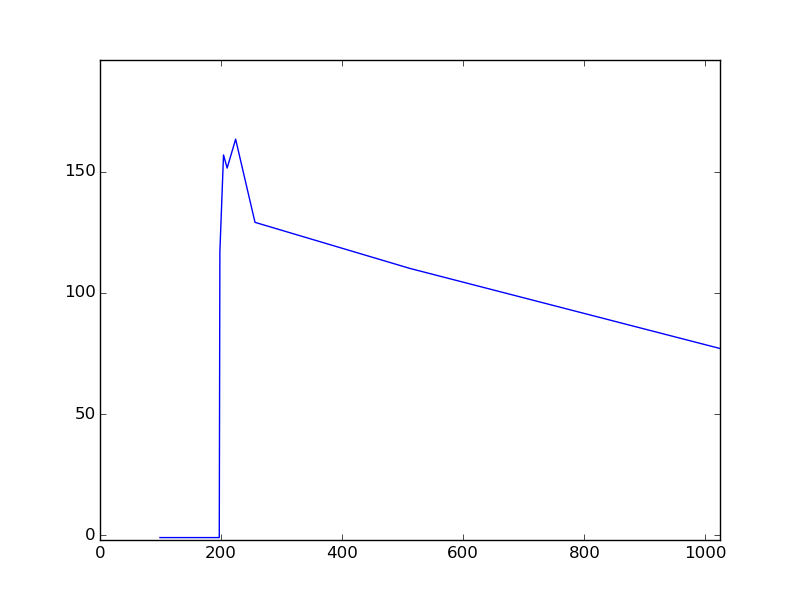
\includegraphics[width=0.5\textwidth]{bintree}}
\subfigure[Pascal Policy]{\includegraphics[width=0.5\textwidth]{pascalbintree}}
\caption{No Restrictions vs. Pascal policy}
\label{pascal}
\end{figure}

Without any restrictions, the memory usage peaks at approximately 700MB while the pascal managed run peaks at approximately 350MB. The memory utilisation is halved but the execution time is increased. Without any restrictions the run takes approximately 30 seconds to complete while the pascal run takes 1 minute and 30 seconds (3 times slower). For comparison reasons, running the same script with a hard heap limit set to the minimum heap size takes 1 minute (2 times slower). The version that uses soft heap limits is slower because it forces the garbage collection to happen more often than the version using hard heap limits.
\\\\
Even though this policy causes the environment to run slower than both an unrestricted one or one that is controlled using hard heap limits, it is a good candidate for comparison as it guarantees that all scripts being managed will execute successfully.
\section{Findings}
\hspace*{3em} Every test scenario was run against each policy in order to measure the isolate \textbf{survival rate} (number of survived isolates vs total number of isolate). At each run the memory budget was slightly increased in order to ease the process of allocating memory. The initial expectancy was to observe growth of survival rate as the memory budget increased. Figure \ref{findings} shows the graph of the survival rates for the 4 policies at each run, the y-axis represents percentage while the x-axis represents the memory budget set for the run.%could set the y axis to be x_min_heap_size, 1 to 2
\begin{figure}[!ht]
  \centering
    \includegraphics[width=0.9\textwidth]{SurvivalRates.png}
    \caption{Survival Rates of each policy}
    \label{findings}
\end{figure}\\
Robin Hood experiences fluctuations in its survival rate, most likely due to the fact that it only redistributes memory between two isolates at any given policy execution. This causes the isolates in between the richest and poorest to remain unattended for potentially long  periods of time, which would lead to their failure. Its unpredictability makes it unsuitable for use in a real system.
\\\\
Inverse throughput also experiences growth as the memory budget is increased, but only reaches a maximum of 99\% survival rate. The fact that the maximum is reached at run 6 and maintained at iteration 7 strongly indicates that any further increases in memory budget will result in diminishing returns. However, the only way to know for certain is through further testing which makes this policy unfeasible because of the unknown (potentially large) budget threshold needed to achieve complete survival.
\\\\
Equal share surprisingly experiences a similar growth in survival rate as Inverse throughput, reaching a maximum of 98\% at run 6 and maintaining it in run 7. However, in the case of this policy, the memory budget needed to achieve 100\% can be calculated and is equal to 5GB. With the current set of tests, it is likely that this policy will slowly increase its survival rate as the memory increases from 840MB to 5GB, which makes is unfeasible.
\\\\
Wealth redistribution is the only policy to successfully run the scenarios with no failed scripts. It exhibits the expected growth in survival rate, starting at 95\% when memory is most constraint and achieving 100\% when the memory budget is equal to double the minimum required heap size(800MB).
\\\\
\hspace*{3em} A memory budget need of double the minimum heap size for successful memory management might seem considerable. However, this needs to be put in perspective in order to effectively determine whether this can be considered a success. To do so, the 12 scenarios were run without any restrictions in order to measure the maximum memory utilisations they achieve as well as an average or the maximum utilisations and an overall average utilisation. Even though the minimum heap size required for every scenario was 400MB, the maximum memory utilisation was 3GB (7.5x minimum heap size) while the average maximum memory utilisation for all scenarios was 1,2GB (3x minimum heap size). Figure \ref{memreduction} is a chart comparing the total memory utilisation running with out restrictions, with pascal policy and with the wealth redistribution policy with 800MB budget:
\begin{figure}[!ht]
  \centering
    \includegraphics[width=0.7\textwidth]{r_finalfindings.png}
    \caption{Memory utilisation comparison}
    \label{memreduction}
\end{figure}
\newpage
From figure \ref{memreduction} it follows that wealth redistribution not only enforces a 800MB memory limit successfully, it also considerably reduces the average maximum memory usage of the scenarios as well as slightly reducing the overall average usage. The argument for deeming this policy effective is that it achieves these results without any prior knowledge of the minimum heap sizes of the scripts it manages. This makes it suitable for real scenarios where it is impractical to attempt to calculate the minimum heap size, especially in the case of websites where the host application is downloaded from the network and its behaviour is highly dependent on user input. Figure \ref{pc_reduction} shows the reduction percentages for each of the 3 measured utilisations.
\begin{figure}[!ht]
  \centering
    \includegraphics[width=0.65\textwidth]{r_averagememreduction.png}
    \caption{Memory reduction comparison (y-axis reduction percentage compared to the unrestricted run)}
    \label{pc_reduction}
\end{figure}\\
While the memory utilisation can be greatly reduced using the wealth redistribution policy, which brings considerable benefits such as reduced memory contention, virtual memory paging avoidance and the potential to increase the multiprogramming degree, execution time is the final factor in evaluating the feasibility of the policy. Figure \ref{time_cmp} shows full test run (all scenarios) execution time in seconds for runs with no restrictions, pascal policy and wealth redistribution.
\begin{figure}[!ht]
  \centering
    \includegraphics[width=0.45\textwidth]{timeanalyze.png}
    \caption{Execution time comparison}
    \label{time_cmp}
\end{figure}\\\\
\hspace*{3em} Wealth redistribution is approximately 20\% slower than the unrestricted run, while Pascal is approximately 50\% slower. This shows wealth redistribution is 2.5 times faster than Pascal and much more memory efficient. The slow down when compared to the unrestricted running time is small enough to be considered unnoticeable to the user as it is only a a fraction of the optimal time. However, there are cases when using the wealth redistribution policy could lead to shorter execution times compared to an unrestricted run. In situations where the maximum utilisation exceeds the available physical main memory the operating system will compensate by using virtual memory. This process requires swapping memory pages between the main memory and permanent storage which slows execution speed considerably. Wealth redistribution can be used to reduce the memory usage of the applications so that it can fit in memory. Compared to an unrestricted run, the memory restricted run would avoid paging and circumvent the implicit delays.
%\begin{figure}[!ht]
%  \centering
%    \includegraphics[width=0.7\textwidth]{r_overallaveragememreduction.png}
%    \caption{Execution time comparison}
%\end{figure}
\section{Summary}
\hspace*{3em} Out of the 4 policies developed, only wealth redistribution managed to obtain a 100\% survival rate using a reasonably small memory budget. It uses the most metrics to calculate isolate welfare and makes the most use of social welfare theory to determine how to divide memory optimally. The memory budget required to achieve complete survival is two times the sum of the minimum heaps of all managed isolates, which is reasonable considering the policy does not know the minimum heap sizes of the running scripts. The applications will experience a 20\% increase in execution when managed by this policy, but this added delay is negligible as it is a sub-unitary fraction of the optimal time.
\chapter{Conclusion}
\hspace*{3em} Inspired by the work of Cameron et al.\cite{forseti} we have devised a memory management framework for the JavaScript ecosystem running on V8. In contrast with previous work, this project strives for generality, aiming to control any kind of garbage collected environment by making limit recommendations regarding the overall heap size of a program. Calculating the minimum heap size of the managed program is impractical, hence the framework uses status metrics collected during execution and applies social welfare theory to determine how to divide memory without causing scripts to fail. To achieve this, various memory management policies have been created and tested using bundles of standard benchmark scripts. The most effective policy was found to be wealth redistribution, managing to achieve a 100\% survival rate with peak footprint reduction of 70\% and average reduction of 55\% while incurring a execution speed decrease of only 20\%. This policy would be useful in a scenario where JavaScript is used to service concurrent clients, as it helps avoid paging, increases the availability (more concurrent servicing applications per node) and does not incur a noticeable performance cost.
\\\\
\hspace*{3em} For the purpose of this project, the Google open source V8 engine has been modified in order to allow external control. A highly modular and extensible control framework has been built in order to track JavaScript applications, calculate and apply memory limits and visualise feedback information about the system. Memory management policies are implemented in separate scripts and can be loaded into the framework at runtime. This allows for easy future research and extensibility without any code re-factoring or modifications. 
\section{Future Work}
\hspace*{3em} The focus of the project was to develop a working framework and an effective policy. This has led to omitting security features in favor of a less complex implementation. These features are normally part of any network based application: 
\begin{enumerate}
\item \textbf{Encription} should be used for any form of communication between the manager and the V8 processes. This would help prevent third parties from simply copying valid protocol packets and reusing them to impersonate either a V8 process or the manager.
\item \textbf{V8 Authentication} - V8 instances would be required to prove their identity before they can be accepted as part of the system and managed by the framework. This would prevent malicious clients from disrupting the memory distribution process by creating fake clients with high memory demands.
\end{enumerate}
\hspace*{3em} Given the success of the wealth redistribution policy and the benefits it has over running concurrent JavaScript applications without any monitoring, future development should focus on improving the performance and scalability of the manager in order to make it suitable for use in the industry (distributed elastic systems). Such improvements include:
\begin{itemize}
\item More \textbf{granular locking} would improve the registry transaction speed. Chapter 5 has presented the locking mechanism used to ensure safe transactions with the registry. This can become a bottleneck when the number of machines starts to increase considerably. In this scenario each update coming from a V8 instance will keep the whole registry locked for the duration of the update servicing call, making it impossible to update in parallel. By moving the lock from a global level to a machine level, updates coming from different machines will be done in parallel, hence reducing the total waiting time.

\item \textbf{Parallel policy execution} - a step further from the optimisation above would be to split the registry on a per machine basis. Policies are applied once for every machine managed by the system. No data regarding any other machine than the one being managed is necessary when applying the policy which allows the process to be done in parallel. This would greatly improve the response time of the manager since the current implementation operates sequentially.

\item \textbf{Single plotter process} - currently the framework uses one plotter process per isolate (because of the plotting library limitations). This means that for each monitored isolate, a plotter separate plotter process visualises and stores its metrics. This can be remedies by using a single plotter process for all tracked isolates and a different live plotting library. Currently, if large numbers of isolates are tracked, the framework can be configured to only plot the aggregate values for each machine using the command ``plotMode MACHINE''

\item \textbf{Automatic budget calculation} - the current implementation allows the system administrator to set a memory budget on a per-machine basis at runtime (using the CLI). In a realistic scenario, the framework would be managing between hundreds and thousands of machines. This makes manual setting of memory budgets impractical. An additional process could be created in order to observe the overall memory utilisation and the total physical memory of each managed node and report back to the manager framework. This information can then be used to automatically calculate and set optimal machine memory budgets.

\item \textbf{Preferential Treatment} - the current version strives for optimal memory allocations that maximise the performance of every managed application. However, in a realistic setting, preferential treatment is a good way of increasing earnings. A good example for this is Amazon Webservices, where higher paying clients receive more computing power.A management policy could be devised to take preferential treatment into account and allocate more memory to applications running for higher paying clients. These clients would experience shorter execution speeds than regular clients.
\end{itemize}
More experimental work can be carried out in the hopes to devise better management policies such as:
\begin{itemize}
\item Collecting \textbf{more metrics} could provide the necessary insight to devise a policy capable of achieving a 100\% survival rate with a budget equal to the minimum heap size, or at least a smaller budget than the current best policy. Some of these metrics could be: average garbage collection time, average execution time, average frequency of garbage collection.
\item \textbf{State based policies} - all policies developed so far are stateless, they do not retain any information about previous iterations. Storing state information could help automatically tune the policy to better adapt to specific characteristics of the environments it manages. The functionality is currently available in the form of a context object passed to the policy execution call.  
\end{itemize}
\hspace*{3em} 
\section{Acknowledgements}
I would like to thank Dr. Jeremy Singer for his feedback and assistance throughout this project and Wing Li for sharing his JavaScript benchmarks.
\begin{appendices}
\chapter{Benchmark Scripts}
The contents...
\chapter{Minimum Heap Size Measurements}
\label{minheapsize}
\begin{figure}[!ht]
  \centering
    \includegraphics[width=0.95\textwidth]{MHCmpBinaryTree.png}
    \caption{Binary Tree Benchmark.}
\end{figure}

\begin{figure}[!ht]
  \centering
    \includegraphics[width=0.95\textwidth]{MHCmpFasta.png}
    \caption{Fasta Benchmark.}
\end{figure}

\begin{figure}[!ht]
  \centering
    \includegraphics[width=0.95\textwidth]{MHCmpKNucleotide.png}
    \caption{KNucleotide Benchmark.}
\end{figure}

\begin{figure}[!ht]
  \centering
    \includegraphics[width=0.95\textwidth]{MHCmpRegexDNA.png}
    \caption{RegexDNA Benchmark.}
\end{figure}
\chapter{Policy Comparison}
Wealth Redistribution for 2 Binarytree benchmarks running in parallel limited at 400MB
\begin{figure}[!ht]
  \centering
    \includegraphics[width=1\textwidth]{binarytree400MLeft.png}
    \caption{Binary Tree 1}
\end{figure}

\begin{figure}[!ht]
  \centering
    \includegraphics[width=0.95\textwidth]{binarytree400Mright.png}
    \caption{Binary Tree 2.}
\end{figure}
\chapter{Findings}
Survival rates for every policy:\\
\begin{tabular}{  | l | l | l | l | l | l | }
\hline  
  Run & Machine Memory Limit & Equal Share & Robin Hood & Inverse Throughput & Wealth Redistribution \\
\hline
  1 & 400MB & 91\% & 84\% & 93\% & 95\%\\
\hline
  2 & 420MB & 93\% & 92\% & 93\% & 97\%\\
\hline  
  3 & 460MB & 96\% & 90\% & 94\% & 96\%\\
\hline  
  4 & 540MB & 95\% & 92\% & 96\% & 97\%\\
\hline  
  5 & 600MB & 97\% & 90\% & 97\% & 99\%\\
\hline  
  6 & 800MB & 98\% & 88\% & 99\% & 100\%\\
\hline
  7 & 840MB & 98\% & 96\% & 99\% & 100\%\\
\hline
\end{tabular}
\\\\
Number of failed scripts out of 440 for every policy:\\
\begin{tabular}{  | l | l | l | l | l | l | }
\hline  
  Run & Machine Memory Limit & Equal Share & Robin Hood & Inverse Throughput & Wealth Redistribution \\
\hline
  1 & 400MB & 38 & 70 & 27 & 19\\
\hline
  2 & 420MB & 28 & 32 & 27 & 11\\
\hline  
  3 & 460MB & 16 & 40 & 24 & 17\\
\hline  
  4 & 540MB & 19 & 34 & 16 & 9\\
\hline  
  5 & 600MB & 9 & 42 & 12 & 4\\
\hline  
  6 & 800MB & 8 & 50 & 2 & 0\\
\hline
  7 & 840MB & 7 & 16 & 2 & 0\\
\hline
\end{tabular}
Averages: equal share:17 robin hood:40 inverse throughput:15 wealth redistribution:8
\\\\
Execution time comparison:\\
\begin{tabular}{  | l | l | l | l | l | l | }
\hline  
  Scenario & Normal Execution Time & Time with Pascal & Time with Wealth Redistribution \\
\hline
  1 & 01:22 & 02:11 & 01:44 \\
\hline
  2 & 02:34 & 04:48 & 04:07 \\
\hline  
  3 & 00:32 & 01:32 & 00:49 \\
\hline  
  4 & 00:20 & 00:21 & 00:20 \\
\hline  
  5 & 02:27 & 03:07 & 03:42 \\
\hline  
  6 & 05:28 & 10:58 & 07:10 \\
\hline
  7 & 00:03 & 00:03 & 00:03 \\
\hline
  8 & 02:04 & 02:06 & 01:22 \\
\hline
  9 & 02:14 & 02:29 & 01:36 \\
\hline
  10 & 05:24 & 06:25 & 07:51 \\
\hline
  11 & 04:38 & 07:07 & 06:44 \\
\hline
  12 & 08:31 & 09:07 & 05:34 \\
\hline
  TOTAL: & 36:00 & 50:00 & 41:00\\
\hline
\end{tabular}

\chapter{Command Line}
\label{allcommands}
\begin{lstlisting}
Manager Commands 
________________________________________________________________________________
>> chhz [frequency in Hz(float)]
Change the machine polling frequency.
>> chv8 [V8Id(int)]
Change the V8 that the shell is set to.
>> dbg
>> echo [0/1 off/on(int)]
Toggle echo function on or off
>> help
   (? ) 
>> history
   (h ) Print command history
>> hz
Get the current polling frequency
>> listPolicies
   (lsp ) List available policies
>> listScenarios
   (listscen lscen ls ) Show a listiong of all scenarios
>> loadConfig [configuration(str)]
   (conf lc ) Load and apply configuration file
>> loadpolicy [policy name(str)]
   (ldp ) Load a difference memory management ploicy.
>> machines
   (m ) Status report of all machines, V8 and isolates.
>> policyname
   (p? ) Configure how the plotters behave, using a JSON string. This is applied to plotters created after this command is issued. options: makePNG(boolean) makeCSV(boolean)
>> policystats
   (ps ) Configure how the plotters behave, using a JSON string. This is applied to plotters created after this command is issued. options: makePNG(boolean) makeCSV(boolean)
>> registryIO
   (rio r? ) Get a summary of the network usage on the registry side
>> run [script(str)]
   (r ) Run a JS script on the V8 the shell is set to.
>> setMachineMemoryLimit [machine_id(str)] [memory_limit_in_MB(int)]
   (mlim ) Set the global memory limit for all JS instances per machine
>> setmax [isolateId(int)] [heap size in bytes(int)]
   (hard ) Set hard limit reccodendation to the isolate from the V8 the shell is set to.
>> setMaxPlotters [max(int)]
   (maxPlt mp ) Set maximum plotter windows allowed
>> setNewMachineMemoryLimit [memory_limit_in_MB(int)]
   (nmlim ) Set the global memory limit for all JS instances for new machines that connect
>> setPlotMode [mode(str)]
   (pmode pm ) Set the plot mode: NONE,MACHINE,ISOLATE,ALL
>> setPlotServerPort [port(int)]
   (plotport pp ) Restart the plotter server on a different port
>> setPlotterStartupConfig [JSON config(str)]
   (pltsconf ) Configure how the plotters behave, using a JSON string. This is applied to plotters created after this command is issued. options: makePNG(boolean) makeCSV(boolean)
>> snapshot [isolateId(int)]
Take a snapshot of an isolate form the V8 the shell is set to.
>> stats
Status report of all machines, V8 and isolates.
>> suggest [isolateId(int)] [heap size in bytes(int)]
   (s soft ) Send hard limmit reccomendation to the isolate from the V8 the shell is set to.
>> switch [machineId(str)] [V8Id(int)]
Change the machine and V8 that the shell is set to.
>> testScenario [path_to_scenario(str)] [path_to_collect_in(str)]
   (scenario rs t ) Run a testing scenario
>> togglePlotServiceLogging [ON/OFF(str)]
   (pslog tpsl ) Toggle PlotService logging
>> v8s
   (v ) Status report of all machines, V8 and isolates.
>> where
What V8 from what machine the shell is set to at the moment.
________________________________________________________________________________
\end{lstlisting}
Strings in () brackets are short forms for the command. 
\end{appendices}

%more accurate biblio
\begin{thebibliography}{9}
\bibitem{intro}
Gregor Richards, Andreas Gal, Brendan Eich, Jan Vitek,
\emph{Automated Construction of JavaScript Benchmarks},
\bibitem{v8gctour}
A tour of the V8 garbage collector,
\url{http://jayconrod.com/posts/55/a-tour-of-v8-garbage-collection},
\bibitem{nodejs}
NWJS Project
\url{http://nwjs.io/}
\bibitem{nwjs}
NodeJS Project
\url{https://nodejs.org/en/}
\bibitem{v8}
V8 Engine
\url{https://developers.google.com/v8/}
\bibitem{spidermk}
SpidermonkeyEngine
\url{https://developer.mozilla.org/en-US/docs/Mozilla/Projects/SpiderMonkey}
\bibitem{chakra}
Chackra Engine
\url{https://github.com/Microsoft/ChakraCore}
\bibitem{forseti}
Callum Cameron, Jeremy Singer, David Vengerov
\emph{The Judgment of Forseti: Economic Utility for Dynamic Heap Sizing of Multiple Runtimes},
\bibitem{powderplayer}
\url{https://github.com/jaruba/PowderPlayer}
\bibitem{whatsap}
\url{https://web.whatsapp.com/}
\bibitem{messenger}
\url{http://messengerfordesktop.com/}
\bibitem{devkit}
\url{https://github.com/printhom/devkit-core}
\bibitem{wunderlist}
\url{https://www.wunderlist.com/download/}
\bibitem{tycoongame}
\url{http://www.greenheartgames.com/app/game-dev-tycoon/}
\bibitem{welfareeconomics}
Deardorff, Alan V. (2014), "Welfare economics", Deardorffs' Glossary of International Economics \url{http://www-personal.umich.edu/~alandear/glossary/w.html#WelfareEconomics}
\bibitem{socialwelfarefunction}
Amartya K. Sen, 1970 [1984], Collective Choice and Social Welfare, ch. 3, "Collective Rationality." p. 33, and ch. 3*, "Social Welfare Functions." \url{http://www.citeulike.org/user/rlai/article/681900}
\bibitem{jsgrandpa}
Naomi Hamilton, “The A–Z of Programming Languages: JavaScript,” Computerworld, July 30, 2008, \url{http://bit.ly/1lKldIe}
\bibitem{jsdaddy}
 Paul Krill, “JavaScript Creator Ponders Past, Future,” InfoWorld, June 23, 2008, http://bit.ly/1lKlpXO; Brendan Eich, “A Brief History of JavaScript,” July 21, 2010, \url{http://bit.ly/1lKkI0M}
\bibitem{github}
GitHub, version control service based on git \hspace*{1em} \url{https://github.com/}
\bibitem{githut}
GitHut, Statistics for GitHub \hspace*{1em} \url{http://githut.info/}
\bibitem{gcpaper}
Paul R Wilson. Uniprocessor garbage collection techniques. In Memory Management, pages 1–42.
Springer, 1992.
\bibitem{v8sizebug}
V8 Maximum Memory Amount Per Isolate
\url{https://bugs.chromium.org/p/v8/issues/detail?id=847}
\bibitem{gc}
1 Automatic Storage Reclamation, Uniprocessor Garbage Collection Techniques, Paul R. Wilson, University of Texas
\bibitem{marksweep}
2.2 Mark-Sweep Collection, Uniprocessor Garbage Collection Techniques, Paul R. Wilson, University of Texas
\bibitem{markcompact}
2.3 Mark-Compact Collection, Uniprocessor Garbage Collection Techniques, Paul R. Wilson, University of Texas
\bibitem{copygc}
2.4 Copying Garbage Collection, Uniprocessor Garbage Collection Techniques, Paul R. Wilson, University of Texas
\bibitem{diminishreturns}
Page 3, Microeconomic Theory,\emph{The Judgment of Forseti: Economic Utility for Dynamic Heap Sizing of Multiple Runtimes}, Callum Cameron, Jeremy Singer, David Vengerov
\bibitem{matplotlib}
Matplotlib library for python
\url{http://matplotlib.org/}
\bibitem{gini}
Gini, C. (1909). "Concentration and dependency ratios" (in Italian). English translation in Rivista di Politica Economica, 87 (1997), 769–789.
\bibitem{ergonomics}
Java Runtime Heap Resizing, Ergonomics,
\url{https://docs.oracle.com/javase/8/docs/technotes/guides/vm/gctuning/ergonomics.html}
\end{thebibliography}
\end{document}